\chapter{Logic}

\begin{flushright}
\emph{An approximate answer to the right question is better than\\
a precise answer to the wrong question.} --- John Tukey (rephrased)
\end{flushright}

$\mathcal{BPZ}$-logic is a hybrid logic combining binary ($\mathcal{B}$), probabilistic ($\mathcal{P}$) and fuzzy ($\mathcal{Z}$) logic\footnote{I use $\mathcal{Z}$ instead of $\mathcal{F}$ to denote fuzziness partly in recognition of Lotfi Zadeh's contributions, and also because $F$ and $f$ are often used for the cumulative distribution function and probability density function in probability theory, which may cause confusion when probabilities and fuzziness are used together.}.  It has both binary and numerical truth values, and is specially designed for AGI (Artificial General Intelligence) \citep*{Goertzel2007} and commonsense reasoning.  The $\mathcal{Z}$ part is a novel approach to vagueness that is slightly different from traditional fuzzy logic.  Emphasis is put on simplicity and efficiency of inference, which is critical to the development of machine learning algorithms.

\footnotesize
* A note on the examples used in this book:  some of them are politically incorrect or somewhat embarrassing.  I prefer examples that are simple, realistic, and relevant to human emotions because they help us think more clearly (cf the Wason selection task).  Usually I just choose the most obvious examples that come to mind.  I'm not trying to be sexist, ageist, sarcastic, etc.
\normalsize

Reasoning under uncertainty is a vast and nightmarishly complex topic in AI.  Simon Parsons's book \citep*{Parsons2001} contains a very good survey of uncertain reasoning, but even that is not exhaustive.  We may look at the following taxonomy of ``ignorance'' proposed by \citep*{Bosc1997} to convince ourselves that $\mathcal{P}$ and $\mathcal{Z}$ are sufficient to represent all forms of commonsense knowledge:
\begin{figure}[H]
\centering
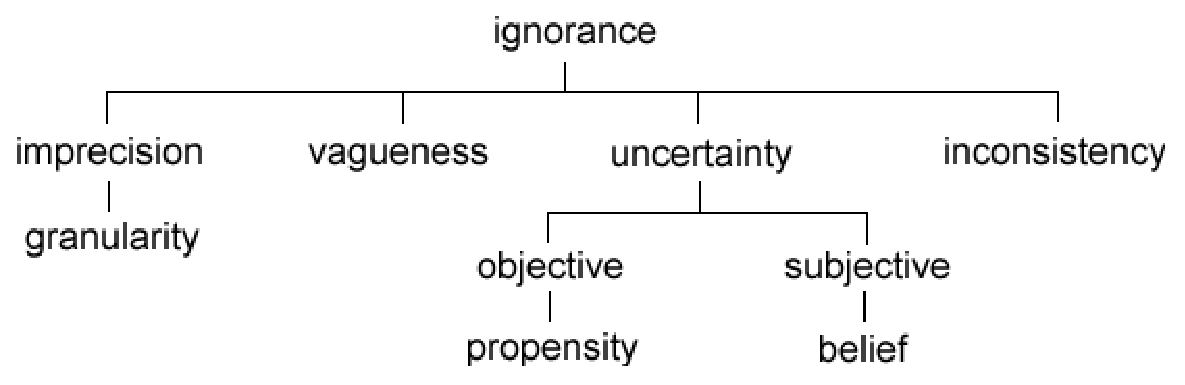
\includegraphics[scale=0.7]{IgnoranceTaxonomy.eps}
\caption{taxonomy of ignorance}
\end{figure}

At first brush, classical logic appears to be sufficient for AGI.  The ability to handle $\mathcal{P}$ and $\mathcal{Z}$ could be made ``emergent'' in the system.  But there are some considerations that make me think that $\mathcal{P}$ and $\mathcal{Z}$ should be built into a seed AGI, particularly because they provide a useful inductive bias to the learning algorithm.  Otherwise, the algorithm would have to learn the rules of fuzzy and probabilistic reasoning from basic arithmetics.  I will give other reasons in \S\ref{sec:whyZ} and \ref{sec:whyP}.

\textbf{Why not include other uncertainty measures besides P and Z?}

There are other theories of uncertainty, such as possibility, belief functions, and rough sets.  The reason I chose $\mathcal{P}$ and $\mathcal{Z}$ is because they are simple and best understood.  There has been attempts to create systems where the user can create a flexible number of uncertainty measures, but one problem of such systems has been pointed out in \citep*{Parsons2001}:  If we have 3 uncertainty measures, say ``cloud'', ``mist'', and ``fog'', there would be a need to provide mixed inference rules for ``cloud-mist'', ``cloud-fog'' etc, a total of $n^2$ possibilities.  I have worked out the mixed rules for $\mathcal{B}$, $\mathcal{P}$ and $\mathcal{Z}$, and have no more appetite for such things unless there is a strong reason to include a new measure.

%With P and Z, the AGI can express ideas such as:\\
%\hspace*{1cm} ``Mary is \underline{probably} \underline{fairly} tall.''

\section{B: binary logic}
\label{sec:binary-logic}

My intuition regarding commonsense reasoning is that it is mainly $\mathcal{B}$, followed by $\mathcal{P}$, and $\mathcal{Z}$ is relatively rare.

It is very important to distinguish between two types of classical logic: \emph{propositional} (zeroth-order) and \emph{first-order}.

A typical propositional statement is:\\
\hspace*{1cm} $ p \vee q \wedge r $\\
whereas a first-order statement is:\\
\hspace*{1cm} $ p(X) \vee q(X,Y) \wedge r(Y) $\\
the chief distinction being the use of \emph{variables} in first-order logic, which greatly increases its expressivity.

%Horn clauses:  P and Z rules can be expressed in Horn form only.  But it seems that we can use general resolution for B rules, no?  Or, perhaps I want to use something similar to Horn resolution for P and Z?

Each rule will enable one inference step, so the logic is almost truth-functional.  The problem is the intermediate results... I only know how to do that in B form.  Maybe we can keep a set of disjunctions of truth values?

In B logic the proof procedure keeps a current clause / or a line of clauses.  In Bayes net we have a query variable and the algorithm finds its P value.  Z logic may be similar to B logic because it's truth functional?

Perhaps we can work out the general case of a query variable of any TV type?  If we draw a B rule that's easy.  If Z rule, then we have a few Z variables as goals.  They need Z rules to fulfill, but what if we have a B rule for one of the sub-goals?  Then we need to translate the B value to Z value.  We can only do that via P(Z).  So we have a P(Z) value as one of the subgoals.  This may cause the head of the rule to become P(Z) too.  It seems there is a tendency for all TVs to become P(Z).
That will actually back-propagate along the proof sequence.

Things may be even worse for a P rule.  The application of the rule requires other numbers.  

\section{Z: fuzzy reasoning}

\subsection{Vague phenomena}

There seems to be 3 types of concepts (= predicates).

The first type is \textbf{discrete} in nature, for example:\\
\hspace*{1cm} sex of a person $\in$ \{ male, female, hermaphrodite, transexual \}\\
\hspace*{1cm} marital status $\in$ \{ single, engaged, married, divorced \}

The second type represents \textbf{numerical} measures, for example:\\
\hspace*{1cm} height \hspace*{1cm} weight \hspace*{1cm} age

The third type is not strictly numerical, but is often associated with ``\textbf{gradedness}'':\\
\hspace*{0.8cm} \begin{tabular}{l l}
beautiful    & ugly\\
intelligent  & dumb\\
simple       & complex\\
interesting  & boring\\
good         & bad\\
easy         & difficult\\
friendly     & hostile\\
clear        & unclear
\end{tabular}

There is no doubt that these predicates can be modified with degrees like ``very'' or ``slightly''.  But we do not know of any exact measures of their degrees.  For example, IQ has been proposed as an inexact measure of intelligence.  Most people would agree that there is some general consensus as to what is intelligent.  Such concepts exhibit \textit{vague phenomena}, which are characterized by:\\
\hspace*{1cm} 1. borderline cases\\
\hspace*{1cm} 2. lack of sharp boundaries\\
\hspace*{1cm} 3. susceptible to sorites paradox\footnote{A solution to the sorites paradox is given in \citep*{Bergmann2008} p268-282, using fuzzy logic and the notion of \textit{decaying validity}.}\\
\hspace*{1cm} 4. open-texture (ie, if $x$ is a borderline case, one can assert either $Q(x)$ or $\neg Q(x)$ in different contexts)

In philosophical logic, there are a number of theories of vagueness (see eg, \citep*{Graff2002}, \citep*{Keefe2000}, \citep*{Shapiro2006}).  $\mathcal{Z}$ logic is a kind of Degree Theory (\citep*{Edgington1992}, \citep*{Sainsbury1986}), that uses numerical truth values to represent vagueness.  There are other non-numerical theories such as Epistemicism (\citep*{Campbell1974}, \citep*{Williamson1994}), and Supervaluation (\citep*{Fine1975}, \citep*{Keefe2000}).

\subsection{Why vagueness is needed for AGI}
\label{sec:whyZ}

One of the critical capabilities of AGI is (self-)programming.  Also, it is imperative to be able to instruct an AGI to write programs according to \textit{natural language} specifications and with robust commonsense background knowledge.  Commonsense reasoning and natural language understanding depend on the use of vague concepts.\footnote{Vague concepts are not required for formal reasoning tasks such as formal mathematics and programming according to formal specifications.}  Look at any (technical or non-technical) natural-language text, and one finds that (explicit or implicit) vague concepts are ubiquitous.  It seems to be occur even more frequently than the (explicit or implicit) use of probabilities.

\textbf{Ubiquity of vagueness in commonsense reasoning.}  Some examples are:\\
\textbullet \, Time: \textit{Mother died \underline{a few days ago}}\\
\textbullet \, Space: \textit{One bird flew \underline{over the cuckoo's nest}} \hspace*{0.5cm} (lacking exact boundaries)\\
\textbullet \, Physics of liquids: \textit{A liquid in bulk and at rest has a horizontal surface}\\ (Is soup a liquid? ``In bulk'' is a fuzzy concept. Is the sea at rest? Surface tension can cause surface to curve)\\
\textbullet \, Physics of solids: \textit{A solid object cannot go from inside to outside a closed box}\\  (``Solid object'' is a fuzzy concept (eg a block of ice, a cat, a bomb). A card box may have small holes. The lid may be slightly ajar.)
%\textbullet \, Minds: 
%\textbullet 
%\textbullet 

\subsection{Why \textit{numerical} vagueness?}

The controversy is whether vagueness should be managed \textbf{quantitatively} (such as $\mathcal{Z}$) or \textbf{qualitatively}.

One objection is that fuzzy logic can sometimes lead to unsound conclusions.  This problem is discussed in \S\ref{sec:exceptions} on nonmonotonic reasoning.

Having numerical vagueness allows us to:\\
1. Represent quantitative rules.  For example:\\
\hspace*{1cm} \begin{tabular}{l l l}
smart & $\leftarrow$ eloquent    & (the more articulate the smarter)\\
      & $\leftarrow$ humorous    & (the more humorous the smarter)\\
      & $\leftarrow$ insightful  & (the more insightful the smarter)\\
      & $\leftarrow$ creative    & (the more creative the smarter)\\
      & $\leftarrow$ etc...      &
\end{tabular}\\
2. Add up graded factors.  For example:\\
\hspace*{1cm} ``John is eloquent, humorous, insightful and creative'' $\rightarrow$ 0.9 smart\\
\hspace*{1cm} ``John is humorous and nothing else'' $\rightarrow$ 0.7 smart\\
3. Accrue contributing factors of a concept over a long period of time:\\
\hspace*{1cm} ``From my long experience with John, he is 0.9 smart''.

On the other hand, if we do not use numerical vagueness, we face these problems:\\
1. Failure to recognize ``partial'' concepts.  For example:\\
\hspace*{1cm} ``John is 0.7 smart'', or\\
\hspace*{1cm} ``cybersex is 0.7 sex''\\
2. Conversely, failure to ignore ``very weak'' partial concepts.\\
3. Each statement must be attached with many qualifications, and they keep accumulating. Each rule would have to recognize a large ``exception set''.

The solution I adopt is to use both qualitative and quantitative information, by representing facts \textit{redundantly} (\S\ref{sec:exceptions}).  For example:\\
\hspace*{1cm} ``John is smart'', $z = 0.7$ (quantitative)\\
\hspace*{1cm} ``But he is only penny wise'' (qualitative)

Lastly, what if we don't need the precision of numerical vagueness in some situations?  For example:\\
\hspace*{1cm} ``Is John really that smart?'' ``Not quite.''\\
or\\
\hspace*{1cm} ``John is slightly smarter than Peter.'' (but we don't know the exact difference)\\
TO-DO:  It seems that we can represent these using $\mathcal{P}(\mathcal{Z})$.

%One suggestion is that we can always use \textit{qualitative} binary statements in place of quantitative ones:\\
%\hspace*{1cm} ``John is fairly intelligent''\\
%\hspace*{1cm} \texttt{intelligent$_1$(john), fairly(intelligent$_1$)}\\
%\hspace*{1cm} ``John is intelligent but only in small matters''\\
%\hspace*{1cm} \texttt{intelligent$_1$(john), qualifies(intelligent$_1$, "only in small matters")}\\
%For the second example, we may say that a person who is intelligent only in small matters is not very intelligent, and thus assign, \textit{eg} Z = 0.6, but some qualitative information would be lost using this numerical representation.

%\begin{tabbing}The following example suggests that at least some \textbf{ordinal} relations may be necessary:\\
%\hspace*{1cm} (A) recently there's been a lot of thefts\hspace*{2cm} \=`that's bad'\\
%\hspace*{1cm} (B) recently there's been a lot of rapes \>`that's very bad'\\
%\hspace*{1cm} (C) recently there's been a lot of murders \>`that's extremely bad' ''
%\end{tabbing}
%which seems to suggest that the severity of crimes has this order:\\
%\hspace*{1cm} theft $<$ rape $<$ murder\\
%but this general ordering can have exceptions depending on circumstances.

%This example shows that sometimes \textbf{quantitative} representations may be necessary:\\
%\hspace*{1cm} ``During the financial crisis,\\
%\hspace*{1cm} (A) many people committed suicide;\\
%\hspace*{1cm} (B) children were sold as prostitutes;\\
%\hspace*{1cm} (C) decades of savings were destroyed''
%So one may react with the feeling ``that's very bad''.  But how was ``\underline{very} bad'' inferred?  Assuming we have a KB that let us infer that:\\
%\hspace*{1cm} A $\rightarrow$ bad\\
%\hspace*{1cm} B $\rightarrow$ bad\\
%\hspace*{1cm} C $\rightarrow$ bad\\
%how can we deduce ``very bad''?  We have 3 heterogeneous contributing factors.  One plausible solution is to assign degrees of badness to each of A, B, and C, and then add them up.

%Note that this example should be a simple reasoning task involving only a few inference steps.

%If the 3 contributing factors \textit{add up} to yield ``very bad'' (even approximately), the individual factors must be \textit{numerical}.  Or, maybe it is a simple counting of contributing factors?  3 bad things?  Not very satisfactory --- the things can have varying degrees.

%``I'm even more sure I don't want to be prostitute, after seeing the bad conditions''.  This is binary.

%But sometimes a rule for a predicate has many antecedents and only some of them are satisfied.  In the binary approach we may qualify them as exceptions.  But there are often many factors that may contribute to a predicate such as $smart$ or $charismatic$.  If you have known John for 10 years there may have been many incidences where he was smart/dumb or charismatic/dull.  In that case we may want to ``add up'' all those contributions.  In other words, it may be desirable to use a single number to summarize a large number of contributions, as long as the contributions are not exceptional.

%Suppose the AGI wants to erect these hypotheses:\\
%\hspace*{1cm} kind $\leftarrow$ attractive\\
%\hspace*{1cm} humorous $\leftarrow$ charismatic

%What if Z is not needed.  All we need is to convert results to binary, qualified form?

%Also, might it be necessary to use numerical Z even for single inference steps?\\
%For example:\\
%sluttish $\rightarrow$ not good wife (Z to Z)\\
%criminal $\rightarrow$ should be punished (Z to Z)\\
%obscene $\rightarrow$ should avoid speaking (Z to Z)\\
%attractive $\rightarrow$ I like (Z to Z)

%During pattern recognition it is often necessary to recognize an entity \textit{partially}, for example, the picture below may be a ``0.7 face''.  It seems that fuzziness is needed at a very fundamental level.
%\begin{figure}[H]
%\centering
%\input{CrossEyesFace}
%\caption{a fuzzy face}
%\end{figure}

\subsection{Semantics of Z}

There is some confusion about the interpretation of fuzziness, which I will try to clarify here.  I am influenced by Pei Wang's ideas \citep*{Wang2006}.

$\mathcal{Z}$ is a measure of \textit{degree} or \textit{gradedness}.  Standard fuzzy theory employs the ``membership function'' to represent \textit{the degree to which an element belongs to a class}, but there is no consensus as to how the membership functions are defined.  Let's think of ``the degree to which a person is smart'', is it really arbitrary?

While there are no exact procedures to measure vague concepts (eg smartness), it is mandatory that a commonsense machine should possess some ways of assessing them, just like the human brain does.  In AGI this can be achieved by having a comprehensive knowledgebase of rules (acquired via machine learning) that compute numerical degrees of concept instances.

Such rules are mini-algorithms (or ``\textbf{micro-theories}'') that are \textbf{emergent properties} of intelligent learning systems.  They establish a \textit{distributed and approximate consensus} of how to measure vague concepts.

If we regard $\mathcal{Z}$ as a measure of degrees, $\mathcal{Z}$ theory is mathematically as rigorous as probability theory.  $\mathcal{Z}$ is a measure of degrees just as the height $H$ is a measure of how tall an object is.  Also, the $\mathcal{Z}$-value can be inexact just as $H$ can be inexact, but this inexactitude is modeled separately by \textit{distributing probabilities over $\mathcal{Z}$} (\S\ref{sec:combinePZ}).

$\mathcal{Z}$ is not an approximation of probability; \S\ref{sec:probabilistic-interpretation} gives a probabilistic interpretation of vagueness, but in practice we can treat $\mathcal{P}$ and $\mathcal{Z}$ as \textbf{orthogonal} to each other.  Possibility theory defines fuzziness as a weaker form of probability (as non-additive probability), but this is not the approach of $\mathcal{Z}$ logic.

Inference in $\mathcal{Z}$ is also different from traditional fuzzy logic (\S\ref{sec:pureZinference}).

\subsection{Probabilistic interpretation of vagueness}
\label{sec:probabilistic-interpretation}

Consider these 2 statements:\\
\hspace*{1cm} A: ``Mary is probably bad-looking''  (with probability $p = 0.8$)\\
\hspace*{1cm} B: ``Jane is rather bad-looking''  (with fuzzy value $z = 0.8$)\\
Suppose John \emph{must} find a pretty girl.  Then he may try Mary, since she has at least a slight chance of being pretty, but definitely not Jane\footnote{``Good-looking'' with $z = 0.2$ means ``bad-looking'', cf \S\ref{sec:gradedness} }.  Thus the 2 statements seem to be subtly different.  Are they really different?

One way to interpret vagueness as probability is to interpret\\
\hspace*{1cm} $Q(x); \; z=z_0$\\
as\\
\hspace*{1cm} ``Among all possible contexts, $Q(x)$ is true with probability $z_0$''.\\
For example, if $smart(john); \; z=0.8$ then John is smart in $80\%$ of circumstances.

Here are more examples:\\
\hspace*{1cm} \begin{tabular}{|l|l|} \hline
\textbf{z = 0.9}             & \textbf{Interpretation}\\ \hline
John is very smart           & John is smart in $80\%$ of circumstances\\ \hline
Peter is very fat            & Peter is fat in $80\%$ of comparisons\\ \hline
Jane is very pretty          & Jane is judged pretty by $80\%$ of beholders\\ \hline
\end{tabular}

%Despite this interpretation, it is easier and more elegant to regard $\mathcal{P}$ and $\mathcal{Z}$ as orthogonal to each other.  For example, if we have a rule that says ``the fatter a person, the clumsier s/he is'', we can represent it with this Bayesian network:
%\begin{figure}[H]
%\centering
%%LaTeX with PSTricks extensions
%%Creator: 0.46
%%Please note this file requires PSTricks extensions
\psset{xunit=.5pt,yunit=.5pt,runit=.5pt}
\begin{pspicture}(188.79882812,70.51660156)
{
\newrgbcolor{curcolor}{1 1 1}
\pscustom[linestyle=none,fillstyle=solid,fillcolor=curcolor]
{
\newpath
\moveto(43.5,20.99999895)
\curveto(43.5,9.68399895)(33.868,0.49999895)(22,0.49999895)
\curveto(10.132,0.49999895)(0.5,9.68399895)(0.5,20.99999895)
\curveto(0.5,32.31599895)(10.132,41.49999895)(22,41.49999895)
\curveto(33.868,41.49999895)(43.5,32.31599895)(43.5,20.99999895)
\closepath
}
}
{
\newrgbcolor{curcolor}{0 0 0}
\pscustom[linewidth=1,linecolor=curcolor]
{
\newpath
\moveto(43.5,20.99999895)
\curveto(43.5,9.68399895)(33.868,0.49999895)(22,0.49999895)
\curveto(10.132,0.49999895)(0.5,9.68399895)(0.5,20.99999895)
\curveto(0.5,32.31599895)(10.132,41.49999895)(22,41.49999895)
\curveto(33.868,41.49999895)(43.5,32.31599895)(43.5,20.99999895)
\closepath
}
}
{
\newrgbcolor{curcolor}{1 1 1}
\pscustom[linestyle=none,fillstyle=solid,fillcolor=curcolor]
{
\newpath
\moveto(176,21.49999895)
\curveto(176,10.18399895)(166.368,0.99999895)(154.5,0.99999895)
\curveto(142.632,0.99999895)(133,10.18399895)(133,21.49999895)
\curveto(133,32.81599895)(142.632,41.99999895)(154.5,41.99999895)
\curveto(166.368,41.99999895)(176,32.81599895)(176,21.49999895)
\closepath
}
}
{
\newrgbcolor{curcolor}{0 0 0}
\pscustom[linewidth=1,linecolor=curcolor]
{
\newpath
\moveto(176,21.49999895)
\curveto(176,10.18399895)(166.368,0.99999895)(154.5,0.99999895)
\curveto(142.632,0.99999895)(133,10.18399895)(133,21.49999895)
\curveto(133,32.81599895)(142.632,41.99999895)(154.5,41.99999895)
\curveto(166.368,41.99999895)(176,32.81599895)(176,21.49999895)
\closepath
}
}
{
\newrgbcolor{curcolor}{0 0 0}
\pscustom[linewidth=1,linecolor=curcolor]
{
\newpath
\moveto(44,21.08302156)
\lineto(132.5,21.41698156)
}
}
{
\newrgbcolor{curcolor}{0 0 0}
\pscustom[linestyle=none,fillstyle=solid,fillcolor=curcolor]
{
\newpath
\moveto(122.5000712,21.37924624)
\lineto(118.51519381,17.36418059)
\lineto(132.5,21.41698156)
\lineto(118.48500555,25.36412363)
\lineto(122.5000712,21.37924624)
\closepath
}
}
{
\newrgbcolor{curcolor}{0 0 0}
\pscustom[linewidth=1,linecolor=curcolor]
{
\newpath
\moveto(122.5000712,21.37924624)
\lineto(118.51519381,17.36418059)
\lineto(132.5,21.41698156)
\lineto(118.48500555,25.36412363)
\lineto(122.5000712,21.37924624)
\closepath
}
}
{
\newrgbcolor{curcolor}{0 0 0}
\pscustom[linestyle=none,fillstyle=solid,fillcolor=curcolor]
{
\newpath
\moveto(13.94042969,15.49999895)
\lineto(13.94042969,17.4335927)
\lineto(22.0078125,27.52050676)
\curveto(22.58072009,28.23663985)(23.12499038,28.85968611)(23.640625,29.38964738)
\lineto(14.85351562,29.38964738)
\lineto(14.85351562,31.24804582)
\lineto(26.1328125,31.24804582)
\lineto(26.1328125,29.38964738)
\lineto(17.29199219,18.4648427)
\lineto(16.3359375,17.35839738)
\lineto(26.390625,17.35839738)
\lineto(26.390625,15.49999895)
\lineto(13.94042969,15.49999895)
\closepath
}
}
{
\newrgbcolor{curcolor}{0 0 0}
\pscustom[linestyle=none,fillstyle=solid,fillcolor=curcolor]
{
\newpath
\moveto(31.41992188,15.49999895)
\lineto(30.36523438,15.49999895)
\lineto(30.36523438,22.22070207)
\curveto(30.11132496,21.97850809)(29.77831748,21.73632083)(29.36621094,21.49413957)
\curveto(28.95409956,21.25194632)(28.58398274,21.07030587)(28.25585938,20.9492177)
\lineto(28.25585938,21.96874895)
\curveto(28.84570123,22.24608595)(29.36132571,22.58202311)(29.80273438,22.97656145)
\curveto(30.24413733,23.37108482)(30.55663702,23.75389694)(30.74023438,24.12499895)
\lineto(31.41992188,24.12499895)
\lineto(31.41992188,15.49999895)
\closepath
}
}
{
\newrgbcolor{curcolor}{0 0 0}
\pscustom[linestyle=none,fillstyle=solid,fillcolor=curcolor]
{
\newpath
\moveto(146.76025391,15.62597551)
\lineto(146.76025391,17.55956926)
\lineto(154.82763672,27.64648332)
\curveto(155.4005443,28.36261642)(155.94481459,28.98566267)(156.46044922,29.51562395)
\lineto(147.67333984,29.51562395)
\lineto(147.67333984,31.37402238)
\lineto(158.95263672,31.37402238)
\lineto(158.95263672,29.51562395)
\lineto(150.11181641,18.59081926)
\lineto(149.15576172,17.48437395)
\lineto(159.21044922,17.48437395)
\lineto(159.21044922,15.62597551)
\lineto(146.76025391,15.62597551)
\closepath
}
}
{
\newrgbcolor{curcolor}{0 0 0}
\pscustom[linestyle=none,fillstyle=solid,fillcolor=curcolor]
{
\newpath
\moveto(160.26708984,19.86230363)
\curveto(160.26708935,20.87792338)(160.37158143,21.69530538)(160.58056641,22.31445207)
\curveto(160.78954976,22.93358539)(161.10009633,23.41112397)(161.51220703,23.74706926)
\curveto(161.92431425,24.0829983)(162.44286842,24.25096688)(163.06787109,24.25097551)
\curveto(163.52880483,24.25096688)(163.9331013,24.15819354)(164.28076172,23.9726552)
\curveto(164.62841311,23.78710016)(164.9155222,23.5195223)(165.14208984,23.16992082)
\curveto(165.36864674,22.82030425)(165.54638094,22.39452343)(165.67529297,21.89257707)
\curveto(165.80419318,21.39061818)(165.86864624,20.71386104)(165.86865234,19.86230363)
\curveto(165.86864624,18.8544879)(165.76513072,18.04101216)(165.55810547,17.42187395)
\curveto(165.35106864,16.80273214)(165.04149863,16.324217)(164.62939453,15.98632707)
\curveto(164.21728071,15.64843642)(163.69677342,15.47949128)(163.06787109,15.47949113)
\curveto(162.23974362,15.47949128)(161.58935365,15.77636598)(161.11669922,16.37011613)
\curveto(160.55029219,17.08495842)(160.26708935,18.24901976)(160.26708984,19.86230363)
\lineto(160.26708984,19.86230363)
\closepath
\moveto(161.35107422,19.86230363)
\curveto(161.35107264,18.45214456)(161.51611153,17.51366893)(161.84619141,17.04687395)
\curveto(162.17626712,16.58007612)(162.58349328,16.34667791)(163.06787109,16.34667863)
\curveto(163.55224231,16.34667791)(163.95946847,16.58105268)(164.28955078,17.04980363)
\curveto(164.61962406,17.51855174)(164.78466295,18.4560508)(164.78466797,19.86230363)
\curveto(164.78466295,21.27636048)(164.61962406,22.21581267)(164.28955078,22.68066301)
\curveto(163.95946847,23.14549924)(163.54833606,23.37792088)(163.05615234,23.37792863)
\curveto(162.57177454,23.37792088)(162.18505618,23.17284296)(161.89599609,22.76269426)
\curveto(161.53271308,22.23925014)(161.35107264,21.27245424)(161.35107422,19.86230363)
\lineto(161.35107422,19.86230363)
\closepath
}
}
{
\newrgbcolor{curcolor}{0 0 0}
\pscustom[linestyle=none,fillstyle=solid,fillcolor=curcolor]
{
\newpath
\moveto(10.41210938,54.49999895)
\lineto(10.41210938,64.40429582)
\lineto(8.70410156,64.40429582)
\lineto(8.70410156,65.90820207)
\lineto(10.41210938,65.90820207)
\lineto(10.41210938,67.12206926)
\curveto(10.41210746,67.88833191)(10.48014125,68.45766728)(10.61621094,68.83007707)
\curveto(10.80240655,69.33136432)(11.13004294,69.73777668)(11.59912109,70.04931535)
\curveto(12.06819305,70.36082293)(12.72525619,70.51658449)(13.5703125,70.51660051)
\curveto(14.11457772,70.51658449)(14.71613962,70.45213143)(15.375,70.32324113)
\lineto(15.08496094,68.6367177)
\curveto(14.68391309,68.70831807)(14.30435617,68.74412533)(13.94628906,68.74413957)
\curveto(13.35904462,68.74412533)(12.94368045,68.61879993)(12.70019531,68.36816301)
\curveto(12.45670177,68.11749835)(12.3349571,67.6484233)(12.33496094,66.96093645)
\lineto(12.33496094,65.90820207)
\lineto(14.55859375,65.90820207)
\lineto(14.55859375,64.40429582)
\lineto(12.33496094,64.40429582)
\lineto(12.33496094,54.49999895)
\lineto(10.41210938,54.49999895)
\closepath
}
}
{
\newrgbcolor{curcolor}{0 0 0}
\pscustom[linestyle=none,fillstyle=solid,fillcolor=curcolor]
{
\newpath
\moveto(23.49609375,55.90722551)
\curveto(22.77993974,55.29850075)(22.09065006,54.86881368)(21.42822266,54.61816301)
\curveto(20.7657816,54.3675121)(20.05500757,54.2421867)(19.29589844,54.24218645)
\curveto(18.04263979,54.2421867)(17.07942461,54.54833874)(16.40625,55.16064348)
\curveto(15.73307179,55.77294689)(15.39648358,56.55533543)(15.39648438,57.50781145)
\curveto(15.39648358,58.06640163)(15.52359934,58.57665502)(15.77783203,59.03857316)
\curveto(16.03206237,59.50048223)(16.36506985,59.87108732)(16.77685547,60.15038957)
\curveto(17.18863674,60.42968052)(17.6523407,60.64094333)(18.16796875,60.78417863)
\curveto(18.5475221,60.88443267)(19.12043819,60.98111226)(19.88671875,61.0742177)
\curveto(21.44790982,61.26040885)(22.59732273,61.48241384)(23.33496094,61.74023332)
\curveto(23.34211366,62.00519977)(23.34569438,62.17349388)(23.34570312,62.24511613)
\curveto(23.34569438,63.03286802)(23.16307738,63.58788048)(22.79785156,63.9101552)
\curveto(22.30370324,64.34699431)(21.56965449,64.56541857)(20.59570312,64.56542863)
\curveto(19.68619283,64.56541857)(19.01480678,64.40607628)(18.58154297,64.08740129)
\curveto(18.14827119,63.76870712)(17.82779625,63.20474284)(17.62011719,62.39550676)
\lineto(15.72949219,62.65331926)
\curveto(15.90136589,63.46255509)(16.18424321,64.11603751)(16.578125,64.61376848)
\curveto(16.97200284,65.11147922)(17.54133821,65.49461686)(18.28613281,65.76318254)
\curveto(19.03092005,66.03172569)(19.89387492,66.1660029)(20.875,66.16601457)
\curveto(21.84895109,66.1660029)(22.64029144,66.05141969)(23.24902344,65.82226457)
\curveto(23.85773814,65.59308681)(24.30532884,65.3048384)(24.59179688,64.95751848)
\curveto(24.87824493,64.61017764)(25.07876556,64.17153875)(25.19335938,63.64160051)
\curveto(25.25780184,63.31216461)(25.29002837,62.71776417)(25.29003906,61.85839738)
\lineto(25.29003906,59.28027238)
\curveto(25.29002837,57.48274336)(25.33120672,56.34586298)(25.41357422,55.86962785)
\curveto(25.4959201,55.39338998)(25.65884311,54.93684747)(25.90234375,54.49999895)
\lineto(23.8828125,54.49999895)
\curveto(23.68228259,54.90104021)(23.55337646,55.37011526)(23.49609375,55.90722551)
\lineto(23.49609375,55.90722551)
\closepath
\moveto(23.33496094,60.22558488)
\curveto(22.63312999,59.93912111)(21.58039667,59.69563177)(20.17675781,59.49511613)
\curveto(19.38183116,59.38052792)(18.81965724,59.2516218)(18.49023438,59.10839738)
\curveto(18.16080373,58.96516375)(17.90657222,58.7556913)(17.72753906,58.47997941)
\curveto(17.54849966,58.20425956)(17.45898152,57.89810753)(17.45898438,57.56152238)
\curveto(17.45898152,57.04589484)(17.65413106,56.61620777)(18.04443359,56.27245988)
\curveto(18.43472924,55.92870845)(19.00585497,55.75683363)(19.7578125,55.75683488)
\curveto(20.50259827,55.75683363)(21.1650325,55.91975664)(21.74511719,56.24560441)
\curveto(22.32518759,56.5714487)(22.75129393,57.01724903)(23.0234375,57.58300676)
\curveto(23.23111116,58.0198522)(23.3349522,58.6643828)(23.33496094,59.51660051)
\lineto(23.33496094,60.22558488)
\closepath
}
}
{
\newrgbcolor{curcolor}{0 0 0}
\pscustom[linestyle=none,fillstyle=solid,fillcolor=curcolor]
{
\newpath
\moveto(32.51953125,56.22949113)
\lineto(32.79882812,54.52148332)
\curveto(32.25455188,54.40690008)(31.76757321,54.34960847)(31.33789062,54.34960832)
\curveto(30.63606392,54.34960847)(30.09179363,54.46061096)(29.70507812,54.68261613)
\curveto(29.3183569,54.90462094)(29.04622176,55.19645007)(28.88867188,55.55810441)
\curveto(28.73111791,55.91975664)(28.65234195,56.68066083)(28.65234375,57.84081926)
\lineto(28.65234375,64.40429582)
\lineto(27.234375,64.40429582)
\lineto(27.234375,65.90820207)
\lineto(28.65234375,65.90820207)
\lineto(28.65234375,68.73339738)
\lineto(30.57519531,69.89355363)
\lineto(30.57519531,65.90820207)
\lineto(32.51953125,65.90820207)
\lineto(32.51953125,64.40429582)
\lineto(30.57519531,64.40429582)
\lineto(30.57519531,57.73339738)
\curveto(30.57519158,57.18196241)(30.60920848,56.82747058)(30.67724609,56.66992082)
\curveto(30.74527605,56.51236672)(30.85627854,56.38704133)(31.01025391,56.29394426)
\curveto(31.16422094,56.2008436)(31.38443557,56.15429417)(31.67089844,56.15429582)
\curveto(31.88573715,56.15429417)(32.16861447,56.17935925)(32.51953125,56.22949113)
\lineto(32.51953125,56.22949113)
\closepath
}
}
{
\newrgbcolor{curcolor}{0 0 0}
\pscustom[linestyle=none,fillstyle=solid,fillcolor=curcolor]
{
\newpath
\moveto(129.39453125,58.67870988)
\lineto(131.29589844,58.43163957)
\curveto(131.08820556,57.12109007)(130.55646781,56.09521219)(129.70068359,55.35400285)
\curveto(128.84488098,54.6127918)(127.79393802,54.2421867)(126.54785156,54.24218645)
\curveto(124.98664916,54.2421867)(123.73160484,54.7524401)(122.78271484,55.77294816)
\curveto(121.83382028,56.79345368)(121.35937414,58.25618008)(121.359375,60.16113176)
\curveto(121.35937414,61.3928957)(121.5634755,62.4706941)(121.97167969,63.3945302)
\curveto(122.37988093,64.3183485)(123.00113682,65.0112189)(123.83544922,65.47314348)
\curveto(124.66975494,65.9350461)(125.57746888,66.1660029)(126.55859375,66.16601457)
\curveto(127.79751874,66.1660029)(128.81086408,65.85268942)(129.59863281,65.22607316)
\curveto(130.38638334,64.59943546)(130.89126565,63.70962515)(131.11328125,62.55663957)
\lineto(129.23339844,62.26660051)
\curveto(129.05435342,63.03286802)(128.73745921,63.60936484)(128.28271484,63.9960927)
\curveto(127.82795491,64.38280156)(127.27831353,64.57616074)(126.63378906,64.57617082)
\curveto(125.65982557,64.57616074)(124.86848521,64.22704)(124.25976562,63.52880754)
\curveto(123.65103852,62.83055702)(123.34667684,61.72590318)(123.34667969,60.2148427)
\curveto(123.34667684,58.68228643)(123.64029634,57.56868077)(124.22753906,56.87402238)
\curveto(124.81477433,56.17935925)(125.58104961,55.83202886)(126.52636719,55.8320302)
\curveto(127.28547499,55.83202886)(127.91926341,56.06477603)(128.42773438,56.53027238)
\curveto(128.93618948,56.99576468)(129.25845478,57.7119098)(129.39453125,58.67870988)
\lineto(129.39453125,58.67870988)
\closepath
}
}
{
\newrgbcolor{curcolor}{0 0 0}
\pscustom[linestyle=none,fillstyle=solid,fillcolor=curcolor]
{
\newpath
\moveto(132.90722656,54.49999895)
\lineto(132.90722656,70.24804582)
\lineto(134.84082031,70.24804582)
\lineto(134.84082031,54.49999895)
\lineto(132.90722656,54.49999895)
\closepath
}
}
{
\newrgbcolor{curcolor}{0 0 0}
\pscustom[linestyle=none,fillstyle=solid,fillcolor=curcolor]
{
\newpath
\moveto(145.32519531,54.49999895)
\lineto(145.32519531,56.1757802)
\curveto(144.43716644,54.88671731)(143.23046192,54.2421867)(141.70507812,54.24218645)
\curveto(141.03189641,54.2421867)(140.40347907,54.37109282)(139.81982422,54.6289052)
\curveto(139.23616253,54.88671731)(138.80289473,55.21077297)(138.52001953,55.60107316)
\curveto(138.23714009,55.99137115)(138.03840982,56.46939802)(137.92382812,57.0351552)
\curveto(137.84505064,57.41470957)(137.80566266,58.01627147)(137.80566406,58.8398427)
\lineto(137.80566406,65.90820207)
\lineto(139.73925781,65.90820207)
\lineto(139.73925781,59.58105363)
\curveto(139.73925447,58.57128394)(139.77864245,57.89094608)(139.85742188,57.54003801)
\curveto(139.97916309,57.03157193)(140.23697533,56.63232103)(140.63085938,56.3422841)
\curveto(141.02473496,56.05224349)(141.51171364,55.9072241)(142.09179688,55.90722551)
\curveto(142.67186873,55.9072241)(143.21613902,56.05582421)(143.72460938,56.35302629)
\curveto(144.23306508,56.65022466)(144.592928,57.05484665)(144.80419922,57.56689348)
\curveto(145.01545362,58.07893417)(145.12108503,58.82193473)(145.12109375,59.79589738)
\lineto(145.12109375,65.90820207)
\lineto(147.0546875,65.90820207)
\lineto(147.0546875,54.49999895)
\lineto(145.32519531,54.49999895)
\closepath
}
}
{
\newrgbcolor{curcolor}{0 0 0}
\pscustom[linestyle=none,fillstyle=solid,fillcolor=curcolor]
{
\newpath
\moveto(150.09472656,54.49999895)
\lineto(150.09472656,65.90820207)
\lineto(151.82421875,65.90820207)
\lineto(151.82421875,64.30761613)
\curveto(152.18228813,64.86619952)(152.65852463,65.31558058)(153.25292969,65.65576066)
\curveto(153.84732553,65.99591844)(154.52408266,66.1660029)(155.28320312,66.16601457)
\curveto(156.12824772,66.1660029)(156.82111813,65.99054735)(157.36181641,65.63964738)
\curveto(157.90249725,65.28872514)(158.28384453,64.79816573)(158.50585938,64.1679677)
\curveto(159.40819236,65.49998795)(160.58267035,66.1660029)(162.02929688,66.16601457)
\curveto(163.16079278,66.1660029)(164.03090909,65.85268942)(164.63964844,65.22607316)
\curveto(165.24835579,64.59943546)(165.55271747,63.63442992)(165.55273438,62.33105363)
\lineto(165.55273438,54.49999895)
\lineto(163.62988281,54.49999895)
\lineto(163.62988281,61.68652238)
\curveto(163.62986783,62.45995192)(163.56720513,63.01675475)(163.44189453,63.35693254)
\curveto(163.31655434,63.69709261)(163.08917826,63.97101812)(162.75976562,64.17870988)
\curveto(162.43032476,64.38638229)(162.04360639,64.49022333)(161.59960938,64.49023332)
\curveto(160.79751389,64.49022333)(160.13149893,64.22345927)(159.6015625,63.68994035)
\curveto(159.07160416,63.15640305)(158.80663046,62.3024)(158.80664062,61.12792863)
\lineto(158.80664062,54.49999895)
\lineto(156.87304688,54.49999895)
\lineto(156.87304688,61.91210832)
\curveto(156.87303865,62.77147505)(156.71548672,63.41600565)(156.40039062,63.84570207)
\curveto(156.08527902,64.27537979)(155.56965453,64.49022333)(154.85351562,64.49023332)
\curveto(154.30923913,64.49022333)(153.80614718,64.34699431)(153.34423828,64.06054582)
\curveto(152.88231998,63.77407821)(152.54752214,63.35513332)(152.33984375,62.80370988)
\curveto(152.13215797,62.25226984)(152.02831693,61.45734876)(152.02832031,60.41894426)
\lineto(152.02832031,54.49999895)
\lineto(150.09472656,54.49999895)
\closepath
}
}
{
\newrgbcolor{curcolor}{0 0 0}
\pscustom[linestyle=none,fillstyle=solid,fillcolor=curcolor]
{
\newpath
\moveto(167.66894531,57.90527238)
\lineto(169.58105469,58.20605363)
\curveto(169.68847387,57.43977465)(169.98746445,56.85253566)(170.47802734,56.44433488)
\curveto(170.96858326,56.03613022)(171.65429221,55.83202886)(172.53515625,55.8320302)
\curveto(173.42317065,55.83202886)(174.08202416,56.01285551)(174.51171875,56.37451066)
\curveto(174.9413983,56.73616207)(175.15624184,57.16047806)(175.15625,57.64745988)
\curveto(175.15624184,58.08430526)(174.96646338,58.42805491)(174.58691406,58.67870988)
\curveto(174.32193277,58.85058053)(173.66307927,59.06900479)(172.61035156,59.33398332)
\curveto(171.19237861,59.69205104)(170.20946944,60.00178381)(169.66162109,60.26318254)
\curveto(169.11376741,60.52456974)(168.69840324,60.88622303)(168.41552734,61.34814348)
\curveto(168.1326486,61.81005023)(167.99120994,62.32030363)(167.99121094,62.8789052)
\curveto(167.99120994,63.38735985)(168.10758352,63.85822526)(168.34033203,64.29150285)
\curveto(168.57307785,64.72476086)(168.88997206,65.08462378)(169.29101562,65.3710927)
\curveto(169.59179428,65.59308681)(170.00178735,65.7810749)(170.52099609,65.93505754)
\curveto(171.04019777,66.0890173)(171.5970006,66.1660029)(172.19140625,66.16601457)
\curveto(173.08658245,66.1660029)(173.87255171,66.03709678)(174.54931641,65.77929582)
\curveto(175.22606598,65.5214723)(175.7255772,65.17235155)(176.04785156,64.73193254)
\curveto(176.37010781,64.29149306)(176.5921128,63.7024637)(176.71386719,62.9648427)
\lineto(174.82324219,62.7070302)
\curveto(174.73729694,63.29426098)(174.48843651,63.75259386)(174.07666016,64.0820302)
\curveto(173.66486963,64.41144737)(173.08300172,64.57616074)(172.33105469,64.57617082)
\curveto(171.4430294,64.57616074)(170.80924097,64.429351)(170.4296875,64.13574113)
\curveto(170.05012715,63.842112)(169.86034869,63.49836234)(169.86035156,63.10449113)
\curveto(169.86034869,62.85383174)(169.93912466,62.62824603)(170.09667969,62.42773332)
\curveto(170.25422851,62.22004331)(170.50129857,62.04816848)(170.83789062,61.91210832)
\curveto(171.03124596,61.8404864)(171.60058133,61.67577302)(172.54589844,61.4179677)
\curveto(173.91373006,61.05272677)(174.86799343,60.75373618)(175.40869141,60.52099504)
\curveto(175.94937255,60.28824185)(176.37368854,59.94986329)(176.68164062,59.50585832)
\curveto(176.98957334,59.06184334)(177.14354454,58.5104116)(177.14355469,57.85156145)
\curveto(177.14354454,57.20702749)(176.95555644,56.6000945)(176.57958984,56.03076066)
\curveto(176.20360407,55.46142377)(175.66112414,55.02099452)(174.95214844,54.7094716)
\curveto(174.24315681,54.39794827)(173.44107428,54.2421867)(172.54589844,54.24218645)
\curveto(171.06347249,54.2421867)(169.93375357,54.5501291)(169.15673828,55.16601457)
\curveto(168.37971866,55.78189871)(167.88378817,56.69498373)(167.66894531,57.90527238)
\lineto(167.66894531,57.90527238)
\closepath
}
}
{
\newrgbcolor{curcolor}{0 0 0}
\pscustom[linestyle=none,fillstyle=solid,fillcolor=curcolor]
{
\newpath
\moveto(179.35644531,50.10644426)
\lineto(179.14160156,51.92187395)
\curveto(179.56412603,51.8072933)(179.93294077,51.7500017)(180.24804688,51.74999895)
\curveto(180.67773169,51.7500017)(181.02148135,51.82161621)(181.27929688,51.9648427)
\curveto(181.53710583,52.10807425)(181.74836864,52.30859489)(181.91308594,52.5664052)
\curveto(182.03482669,52.75976631)(182.23176659,53.23958354)(182.50390625,54.00585832)
\curveto(182.53970899,54.11328058)(182.5970006,54.27083251)(182.67578125,54.47851457)
\lineto(178.34667969,65.90820207)
\lineto(180.43066406,65.90820207)
\lineto(182.8046875,59.30175676)
\curveto(183.11262509,58.46386217)(183.38834096,57.58300367)(183.63183594,56.65917863)
\curveto(183.85383528,57.54719642)(184.11880898,58.41373201)(184.42675781,59.25878801)
\lineto(186.86523438,65.90820207)
\lineto(188.79882812,65.90820207)
\lineto(184.45898438,54.30663957)
\curveto(183.99348358,53.05338581)(183.6318303,52.19043094)(183.37402344,51.71777238)
\curveto(183.0302684,51.08040601)(182.63638858,50.61312132)(182.19238281,50.31591691)
\curveto(181.74836864,50.01872087)(181.21842125,49.87012076)(180.60253906,49.87011613)
\curveto(180.23014099,49.87012076)(179.81477682,49.94889673)(179.35644531,50.10644426)
\lineto(179.35644531,50.10644426)
\closepath
}
}
\end{pspicture}

%\caption{Bayesian network with Z-valued nodes}
%\end{figure}
%where the nodes are $\mathcal{Z}$-valued (continuously valued).  

There are 2 problems with this interpretation:\\
1.  Concerning the min-max calculus (\S\ref{sec:min-max-VS-sum-product})\\
2.  If John has seen Jane and judged her to be 0.2 pretty, then there seems to be no uncertainty about it in this context (John being the judge and Jane having her present looks, etc).  So if John really must find a 0.9 pretty girl then he should prefer Mary (whom he hasn't met and has p=0.2 of being pretty).  The difference is real if we admit that pretty is a matter of degree.

\subsection{Reference classes}

The measure of a $\mathcal{Z}$ value is dependent upon its \textit{reference class}.  For example, if we want to say how ``young'' a person is, the reference class may be ``all people'' or ``all tenured professors''.  The measure of ``youngness'' thus varies depending on the reference class.

Once the reference class is fixed, it seems that $\mathcal{Z}$ is \textit{not} context-dependent.  For example, we can say ``John is a young man who owns an old dog''.  The dog is described as ``old'' using its own reference class (dogs), not John's reference class (humans).

\subsection{Numerical scale of Z}
\label{sec:gradedness}

Many ``natural'' quantities occur in the range $[0,\infty)$.  For example, the height, weight, age, or ugliness of a person can theoretically range from 0 to $\infty$.  It is unnatural to set artificial upper limits to these measures.  However, it may be possible to extend these concepts to the range $(-\infty,\infty)$.  For example, the age of AGI may be $\sim-10$ because it is not yet born.  I reserve this possibility but will use $[0,\infty)$ for now.

$\mathcal{Z}$ is defined in $[0,1]$.  So we need \textbf{membership functions} to map $[0,\infty)$ to $[0,1]$.  I choose a sigmoid function with parameter $\xi$ because it has some nice properties.  We need two orientations because some concepts get more and more positive as $x \rightarrow \infty$, while others the opposite.
\begin{equation}
Z_1(x) = e^{{-\ln 2 \, x^2}/{\xi^2}} \quad \mbox{and} \quad Z_2(x) = 1-e^{{- \ln 2 \, x^2}/{\xi^2}} 
\end{equation}
\begin{figure}[H]
\centering
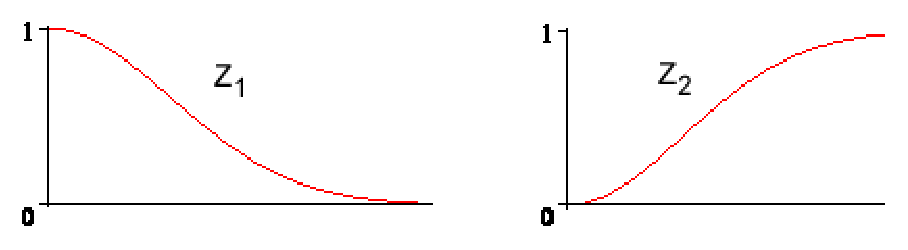
\includegraphics[scale=0.7]{MappingFunctions.eps}
\caption{membership functions}
\end{figure}

\textbf{Negation} is defined as $1-z$.  As a consequence of this, for any concept, $z = 0$ means the \textit{antithesis} of that concept.  For example Z(young) = 0 would mean ``old''.  Another consequence is that the point at $z = 0.5$ is the \textbf{point of neutrality}, which is where a concept is neither true nor false.

The interpretation of the parameter $\xi$ is that \textit{it is the point of neutrality on the x-axis}.  This is illustrated as follows:  we map the human age $x$ to the $\mathcal{Z}$-concept of ``young'', where I subjectively define ``40 years old'' as the neutral point:
\begin{figure}[H]
\centering
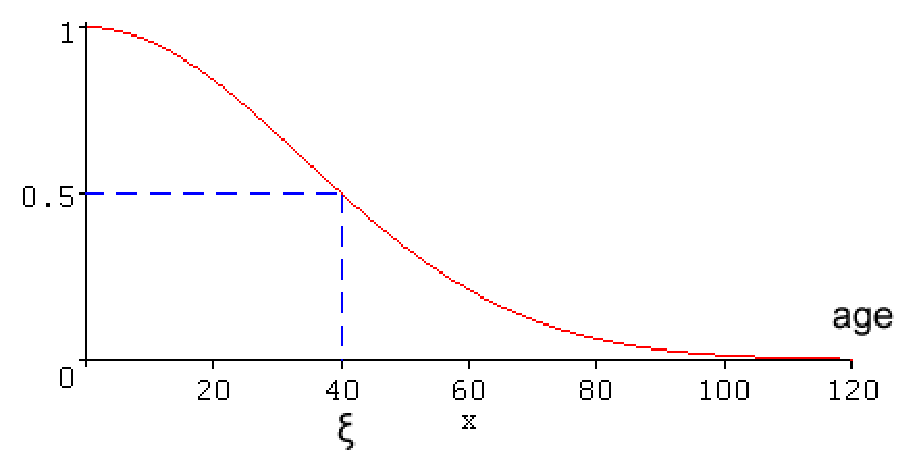
\includegraphics[scale=0.5]{NeutralPoint.eps}
\caption{neutral point}
\end{figure}
That means, after 40, one gets more and more ``not young'' according to this definition.  (Cf \S\ref{sec:exceptions} about exceptions handling.)

Thus the numerical scale of $\mathcal{Z}$ is:\\
\begin{table}[H]
\parbox{3cm}{\caption{}}
\begin{tabular}{|l||l|}
\hline
{\bfseries z} & {\bfseries interpretation}\\ \hline
1.0     & definitely or extremely\\
0.9     & very\\
0.7-0.8 & moderately\\
0.6     & slightly\\ \hline
0.5     & neutral\\ \hline
0.4     & slightly not so\\
0.3-0.2 & moderately not so\\
0.1     & very not so\\
0.0     & definitely or extremely not so\\ \hline
\end{tabular}
\end{table}

\subsection{Why Z obeys min-max calculus}
\label{sec:min-max-VS-sum-product}

Probabilities obey sum-product calculus;  $\mathcal{Z}$ obeys \textbf{min-max calculus} \citep*{Zadeh1965}.  My justification for min-max is as follows:

As an example, consider the statement:\\
\hspace*{1cm} S1: \textit{``John have had sex with 1000 women''}\\
but it turns out that all those women had only had cybersex with him.  Most people would agree that cybersex is not quite the same as real sex (it's a borderline case).  Suppose we subjectively think that cybersex is 0.7 real sex (as a measure of degree), then what would be the ``degree of truthfulness'' of the statement S1 (assuming that we accept the fact that he had cybersex with 1000 women)?

If we use the sum-product calculus (as with probabilities), the answer would be $ 0.7^{1000} $ which is almost zero.

Whereas if we use the min-max calculus, the answer would be $min\{0.7, 0.7, ...\} = 0.7$.  So, did John have sex with 1000 women?\\
\hspace*{1cm} answer A:  ``Of course not.''\\
\hspace*{1cm} answer B:  ``Well... sort of.''\\
My view is that the conjunction of 1000 vague events should have the same vagueness as the individual events.  You may try this with other examples of graded events.

%If this is still unclear, consider more examples:\\
%\hspace*{1cm} S2: ``John ate 100 hotdogs in 1 hour'' (but they are all mini-hotdogs)\\
%\hspace*{1cm} S3: ``John defeated 20 chessmasters'' (but they each offered him 2 free moves)\\
%\hspace*{1cm} S4: ``John is fluent in 20 languages'' (but they are computer programming languages)\\
%\hspace*{1cm} S5: ``John finished reading 50 novels'' (but they are all abridged versions)\\
%Would you accept these statements as \textit{partially} true?  Min-max calculus would grant that they are ``somewhat'' true.  Sum-product, however, would infer that they are effectively completely false.

\subsection{A fuzzy paradox}

A common problem in fuzzy logic is concerning the truth value of statements such as ``Q and not Q''.  It can be resolved using our understanding of $\mathcal{Z}$ negation:

Suppose $Z(tall(john)) = 0.6$ (which means that John is slightly tall)\\
then\\
\hspace*{1cm} $ tall(john) \wedge \neg tall(john) = 0.4$ (which means this is slightly false)\\
\hspace*{1cm} $ tall(john) \vee \neg tall(john) = 0.6$ (which means this is slightly true)

On the other hand, if $Z(tall(john)) = 0.4$ (which means that John is slightly short)\\
then\\
\hspace*{1cm} $ tall(john) \wedge \neg tall(john) = 0.4$ (which means this is slightly false)\\
\hspace*{1cm} $ tall(john) \vee \neg tall(john) = 0.6$ (which means this is slightly true)

All these are reasonable conclusions.

\subsection{``Soft'' MIN-MAX and concept learning}

As an example, let's consider the concept ``human'' for which there can be many exemplars: male, female, baby, child, adult, tall, short, fat, thin, etc.  Suppose we are given the following logical knowledgebase:\\
\hspace*{1cm} human $\leftarrow$ short hair, male face, torso, flat chest, 2 arms, 2 legs, penis\\
\hspace*{1cm} human $\leftarrow$ long hair, female face, torso, breasts, 2 arms, 2 legs, vagina\\
then at least we need to have a knowledge representation scheme capable of representing:

\hspace*{1cm} \begin{tabular}{|l|l|l|} \hline
\textbf{features}           & \textbf{degree} &\\ \hline
(no penis) $\wedge$ vagina  & 1.0             & typical female\\
(no vagina) $\wedge$ penis  & 1.0             & typical male\\
penis $\wedge$ vagina       & 0.6             & hermaphrodite (atypical human)\\
\hline
\end{tabular}

It seems that ``penis'' and ``vagina'' are both contributing factors to ``human'', but paradoxically their conjunction results in an atypical instance.  ``Crisp'' min-max would be unable to represent this, so I created a ``soft'' version of min-max (the idea is to use $z_1, z_2$ as their own weights in a weighted average):

%Is soft required?  We need nonlinear to take care of hermaphrodite?

\hspace*{1cm} \begin{tabular}{|l|l|}
\hline
{\textbf{soft MIN (= AND)}} & {\textbf{soft MAX (= OR)}}\\ \hline
\rule[-7mm]{0mm}{16mm} 
$\displaystyle z_1 \; \widetilde{\wedge} \; z_2 = \frac{z_1 (1-z_1) + z_2 (1-z_2)}{1 - z_1 + 1 - z_2} $
& $\displaystyle z_1 \; \widetilde{\vee} \; z_2 = \frac{z_1 z_1 + z_2 z_2}{z_1 + z_2} $ \\
\hline
\end{tabular}
\parbox{4cm}{\begin{equation}
\label{eqn:soft-MIN-MAX}
\end{equation}}

It can be verified that soft-MIN and MAX satisfy the boundary conditions of classical logic, provided that we make $0/0 = 1$ in the MIN case.

\begin{figure}[H]
\centering
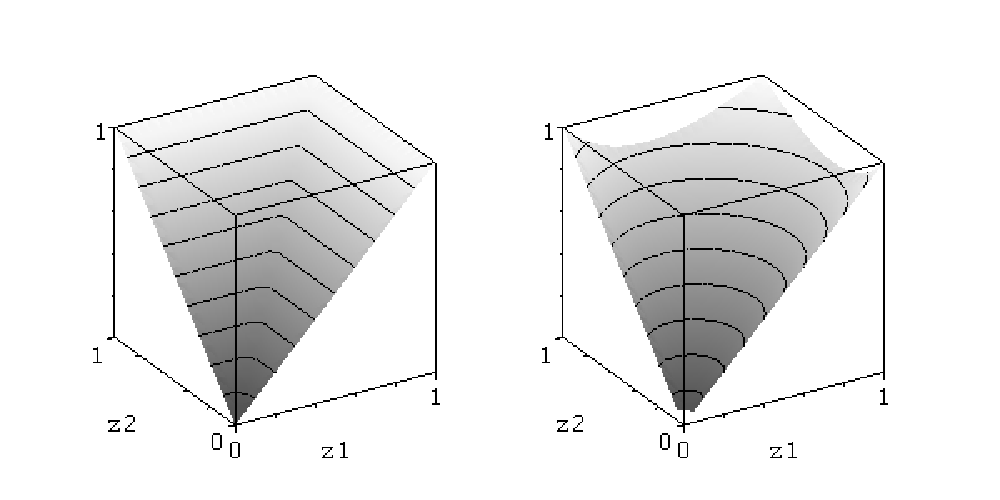
\includegraphics[scale=0.7]{soft-max.eps}
\caption{comparison of MAX and soft MAX}
\end{figure}

\{ TODO:  Is soft min-max really needed, and why?  The current argument is a bit unclear. \}

\subsection{Z modifiers}

To make $\mathcal{Z}$ logic more versatile, we need to augment it with \textbf{hedges} which correspond to natural language words like:\\
\hspace*{1cm} extremely \hspace*{1cm} very \hspace*{1cm} moderately \hspace*{1cm} slightly\\
so we can express things like:\\
\hspace*{1cm} $\mbox{lukewarm} \leftarrow \mbox{moderately(warm)}$\\
\hspace*{1cm} $\mbox{obese} \leftarrow \mbox{very(fat)}$

In general, we can define a $\mathcal{Z}$-modifier as a function $\Gamma: [0,1] \rightarrow [0,1]$,
\begin{equation}
z_0 := \Gamma(z_1)
\end{equation}
We further restrict the class of $\Gamma$ to make the system simpler.  I suggest to use Gaussian functions with the mean $z^*$ as a parameter, and the variance would be fixed to a certain constant.  So
\begin{equation}
z_0 := \Gamma(z_1; z^*_1)
\end{equation}
For example, the $\Gamma$'s for ``slightly'' and ``very'' can be:
\begin{figure}[H]
\centering
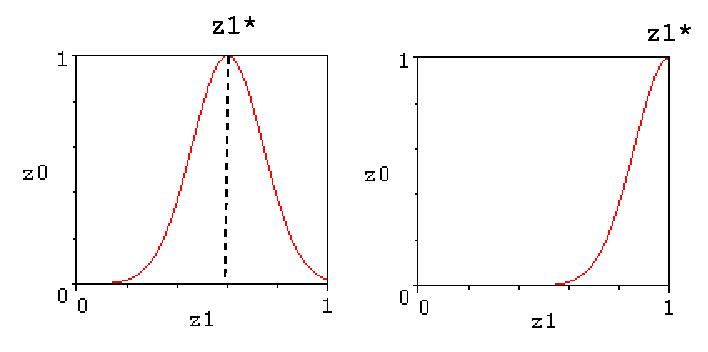
\includegraphics[scale=0.7]{fuzzy-modifiers.eps}
\caption{Fuzzy modifiers with $z^* = 0.6, 1.0$}
\end{figure}

We can have better control over the shapes of $\Gamma$ by using other functions and having more parameters (cf \S\ref{sec:unified-BPZ-inference}), but I suspect that such sophistication is not needed for commonsense reasoning.

For example, we can define ``lukewarm'' as ``warm'' with $z \in [0.6,0.8]$, or:\\
\hspace*{1cm} $\mbox{lukewarm} \leftarrow \Gamma_{0.6}(\mbox{warm}) \wedge \Gamma_{0.8}(\mbox{warm})$\\
using 2 $Gamma$'s with fixed variances.  The result is the blue curve on the left.  We get the interval [0.6,0.8] by taking $> 0.5$ as true, and thus ``lukewarm'' would be a binary predicate.
\begin{figure}[H]
\centering
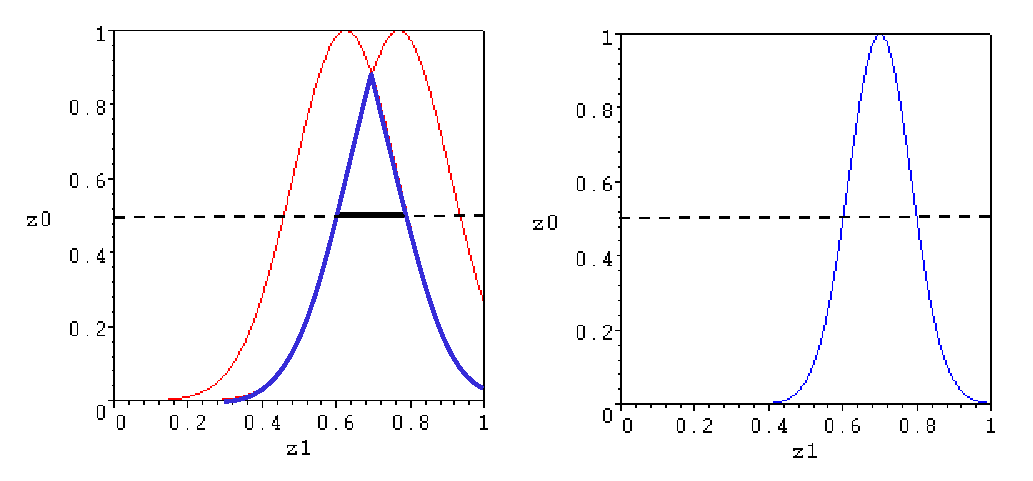
\includegraphics[scale=0.7]{Gamma-for-lukewarm.eps}
\caption{Two representations of ``lukewarm''}
\end{figure}
On the other hand, if we use a tailored $\Gamma$ to represent ``lukewarm'' on the right, it would be a $\mathcal{Z}$-predicate with continuous values like ``slightly lukewarm'' and ``very lukewarm''.  This seems to be unnecessarily sophisticated.

TO-DO:  Prove that combinations of $\Gamma$ and $\widetilde{\vee} \; \widetilde{\wedge}$ can be universal approximators.

\subsection{Z rules and Z inference}

$\mathcal{Z}$ inference is driven by $\mathcal{Z}$ rules.  A $\mathcal{Z}$ rule is specified by a combination of soft MIN's and MAX's (similar to DNFs (disjunctive normal forms) in classical logic):
\begin{equation}
z_0 \; := \; \widetilde{\bigvee_i} \; \widetilde{\bigwedge_j} \; \Gamma(z_{ij})
%z_0 \; := \; \widetilde{\bigvee_i} \; \widetilde{\bigwedge_j} \; \Gamma(z_{ij}; z^*_{ij}, v_{ij}) \, = \; \widetilde{\bigvee} \; \{ z_{11} \, \widetilde{\wedge} \, z_{12} \, \widetilde{\wedge} \cdots, z_{21} \, \widetilde{\wedge} \, z_{22} \, \widetilde{\wedge} \cdots, \, \cdots \}
\end{equation}

Notice that a $\mathcal{Z}$ rule directly assigns a $\mathcal{Z}$ value to $z_0$ \textit{without the use of an implication operator}, which is very different from traditional fuzzy logics.

\subsubsection{Traditional fuzzy logic}

A fuzzy implication is a map $\Rightarrow: [0,1] \times [0,1] \rightarrow [0,1]$ satisfying these boundary conditions from binary logic:\\
\hspace*{1cm} \begin{tabular}{|l|l|l|} \hline
$\Rightarrow$ & 0 & 1\\ \hline
0             & 1 & 1\\
1             & 0 & 1\\ \hline
\end{tabular}

A fuzzy implication statement:  $(Z_1 \wedge Z_2) \Rightarrow Z_0$  means that the fuzzy values $z_0,z_1,z_2$ obey the equation:
$$ ((z_1 \wedge z_2) \Rightarrow z_0) = z_c $$
where $z_c$ is the truth value of the implication statement.  Compared to my approach, this has an extra level of indirectness.  Is it really necessary that we know the truth value of an implication statement?  (Cf \S\ref{sec:P-and-ClassicalLogic}: In probabilistic logic, the probability conditional $P(A|B)$ serves as the implication statement, but we usually do not ask about its own probability.)  One trouble with traditional fuzzy logic is that we cannot even perform \textit{modus ponens} unless we allow interval fuzzy values.\footnote{Suppose we define the operators for a very simple fuzzy logic: $a \Rightarrow b \equiv \neg a \vee b$, $\neg a \equiv 1-a $, and $a \vee b \equiv min(a,b)$.  \citep*{Kenevan1992} has given an inference algorithm for this logic, but it is very complicated and involves interval fuzzy values, and thus unsuitable for machine learning.}

% Now given that $Z_1 = z_1$ and $Z_1 \Rightarrow Z_0$, ie $ (z_1 \Rightarrow z_0) = z_c $, ie $min(1-z_1,z_0)=z_c$ we still cannot determine $z_0$.}

% TO-DO:  weighted soft min-max may not be needed, if we have fuzzy modifiers

%An example involving vagueness: ``smart''\\
%\hspace*{1cm} smart $\leftarrow$ humorous\\
%\hspace*{1cm} smart $\leftarrow$ articulate\\
%\hspace*{1cm} smart $\leftarrow$ blah

\subsection{Z abduction}

TO-DO:  unfinished.

%Z abduction sometimes gives out-of-bounds Z values.\\
%\hspace*{1cm} $ z_1 \widetilde \vee z_2 = high $\\
%\hspace*{1cm} $ z_1 = low $\\
%\hspace*{1cm} $ \Rightarrow z_2 > 1.0 $
%
%Also, there are always 2 solutions, and they are within-bounds in the $z_1 > 0.5$ regime. Why?
%
%In fact, abduction using a rule with a point-Z-value is very unnatural.  Perhaps if we use $P(Z)$ the problem will be resolved?  But the ``2 roots'' problem seems to remain...

\subsection{Z inference algorithm}
\label{sec:pureZinference}

$\mathcal{Z}$ inference (Algorithm \ref{algorithm1}) is analogous to backward-chaining in binary logic (such as Prolog), except that it calculates the $\mathcal{Z}$ value of the query.

\begin{algorithm}
\caption{backward-chaining Z inference}
\label{algorithm1}
\begin{algorithmic}[1]

\REQUIRE a knowledgebase $KB$, a list of query goals $G$ \\
\ENSURE $z =$ the truth value of $G$.

\REPEAT
	\STATE choose a literal $L$ from the list $G$, removing it from G
	\STATE find a rule $z_0 := \widetilde{\bigvee} \widetilde{\bigwedge} z_{ij} $ such that\\
			 $L$ unifies with the consequent $z_0$ \\
	\COMMENT{ if $z_{ij}$ is null, $z_0$ is a fact in $KB$ }
	\STATE add the rule's antecedents ($z_{ij}$) to the list $G$ \\
	\STATE if depth of recursion $< h$ \\
			 recurse to resolve the new list of goals $G$ \\
\UNTIL{ there are no more applicable rules in $KB$. }

\end{algorithmic}
\end{algorithm}

TO-DO:  include $\mathcal{Z}$-abduction.

\subsection{Handling exceptions (nonmonotonic reasoning)}
\label{sec:exceptions}

Fuzzy reasoning can sometimes lead to unsound conclusions, for example:\\
\textit{1. Mary has cybersex with many partners.\\
2. Cybersex is a kind of sex.\\
3. Therefore, Mary has many sex partners.\\
4. A person who has many sex partners has a high chance of STDs.\\
5. Therefore, Mary has a high chance of STDs.}

What's wrong with this example?  On the one hand, we should admit that cybersex is sex (it is a borderline case), but it lacks certain prominent features of sex, such as physical contact (which is not necessarily a \textit{defining} feature of sex).  Thus, if we carry on reasoning with the idea that cybersex is sex, we may get unsound conclusions.  The key to resolving this problem is to recognize ``cybersex is sex'' with \textbf{qualifications} such as ``but it is sex without physical contact''.

If we have a rule saying that ``sex transmits certain diseases'', we may have to attach the exception ``only if the sex involves physical contact''.  In the end, our rules may be inundated with possibly infinitely many exceptions.  How can we get out of this problem?

\citep*{Wang1994}, \citep*{Wang2006} provided a solution, which I essentially adopt.  His idea is not to store the exceptions to rules, but instead allow a \textit{multitude} of rules to fire, calculate the ``confidence'' (\S\ref{sec:NARSconfidence}) of each conclusion, and pick the conclusion with the highest confidence.  This allows us to handle exceptions relatively easily.

Some more examples:\\
\hspace*{1cm} \textbullet \textit{ Age, sex, etc, should not be basis for discrimination.}\\
\hspace*{1cm} \textbullet \textit{ Hermaphrodites are atypical, but no less human than other people.}\\
\hspace*{1cm} \textbullet \textit{ Penguins are birds but they cannot fly.}

%``Nonmonotonic'' means that, when you add a statement to a KB (knowledgebase), some of the earlier conclusions of the KB may no longer be valid.

%For example, you may have a Prolog rule that says:\\
%\hspace*{1cm} \ttfamily fly(X) :- bird(X). \rmfamily\\
%but you may also add an \emph{exception} to this rule:\\
%\hspace*{1cm} \ttfamily fly(X) :- penguin(X), !, fail. \rmfamily\\
%which means that if penguin(X) is true, fly(X) would fail.\\
%The application of the second rule...

\subsection{Doing B inference as Z inference}

TO-DO:  There is a possibility of performing all reasoning in pure $\mathcal{Z}$-logic.  Might it be more advantageous than a hybrid $\mathcal{BPZ}$ logic...?

%$patriot \curlyvee traitor = 0.8$\\
%$\neg patriot \Rightarrow z(patriot) = 0.25$

\section{P: probabilistic reasoning}

For an excellent introduction to probabilistic reasoning and Bayesian networks, see Judea Pearl's book \citep*{Pearl1988}.

\subsection{Why P is needed}
\label{sec:whyP}

In machine learning it is often necessary to learn facts that are only \textit{contingently true}, such as the fact that ``females often have long hair''.  Learning algorithms typically need to keep track of the frequencies of how often the hypotheses are true, in order to pick the highly probable ones.  So it seems that probabilistic logic should be built into the knowledge representation.

\subsection{Positive and negative evidence, and confidence}
\label{sec:NARSconfidence}

Pei Wang's uncertain logic is particularly elegant.  I adopt two ideas from his theory, explained below, but the way I use those numbers differs slightly from Wang's (cf his book \citep*{Wang2006} which describes an AGI called NARS (Non-axiomatic Reasoning System)).

{\bfseries Positive and negative evidence.}  In Wang's logic, each statement is attached with 2 numbers: the number of positive ($w^+$) and negative ($w^-$) examples.  In an AGI system, they are the number of times a statement is observed to be true or false, respectively.

For example, for the statement\\
\hspace*{1cm} ``if X is female X probably has long hair''\\
the AGI may have observed 70 females with long hair and 30 females with short hair. The total support for the statement would be $(w^+ + w^-) = 100$ examples.

Using a pair of numbers allows us to know the probability of a statement as well as the the number of examples that support that statement. This is very important because some statements may be supported by very few examples and thus are ``weaker'' than statements with more support.

A major advantage of this 2-number approach is that probabilities can be updated by new examples. For example, if the AGI encounters a new female with long hair, it can update the probability easily with $ (w^+ + 1,w^-)$. Such updating cannot be done with the single-number representation of probability.

{\bfseries Confidence.}  In NARS, the confidence of a statement is a measure of its \emph{support}, ie, the size of $ w = w^+ + w^- $, or how many examples (positive and negative) that support the statement.

We can map w to the $[0,1]$ interval using some transform.

The frequency (or probability) of the statement is simply:
\begin{equation}
f = p = \frac{w^+}{w}
\end{equation}
Thus, $(w^+,w^-)$ contains information equivalent to the frequency and confidence $ (f,c) $.

\subsection{Gaussian and Beta distributions}

One very useful fact for designing AGI is that many quantities that occur naturally in our physical world seem to obey Gaussian distributions.  This follows from the Central Limit Theorem which states that the sum of a large number of independent and identically-distributed random variables will be approximately normally distributed.

The upshot of this is that the majority of fuzzy quantities, such as tallness, can be represented using Gaussian distributions.  For example, the height of an unknown woman may have a Gaussian distribution with a mean of ``5 feet 4''.  So we can just use 2 numbers, the mean and variance, to represent the distribution, instead of using a table which takes up more memory.

Since $\mathcal{Z}$ values are defined within $[0,1]$, we can use the Beta distribution which is a very versatile distribution:

\begin{figure}[H]
\centering
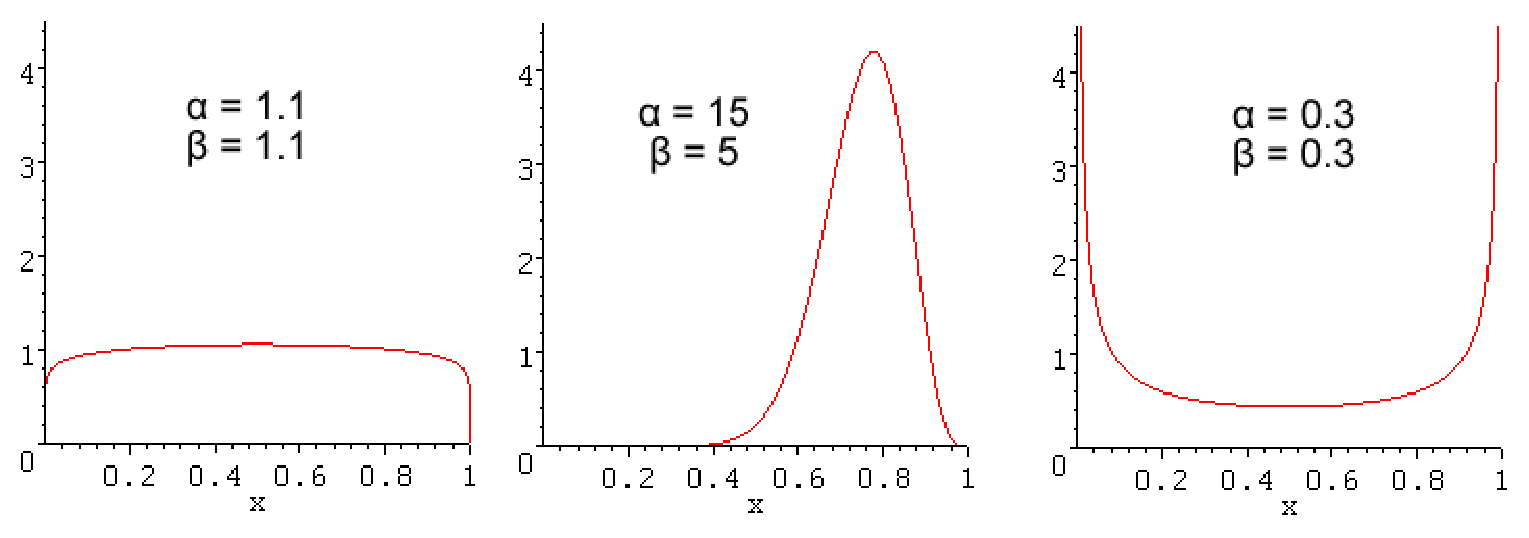
\includegraphics[scale=0.65]{BetaDistributions.eps}
\caption{some shapes of the Beta distribution}
\end{figure}

\begin{enumerate}
\item The first graph shows an almost uniform distribution, which represents a high amount of uncertainty. (If $ \alpha = \beta = 1 $ one gets the uniform distribution.)
\item The second graph is unimodal.
\item The third graph shows an inverted bell curve.  It may be useful for representing distributions such as ``unhealthiness'' over body weights (people who are too thin or too heavy are unhealthy).
\end{enumerate}

Sandy Zabell \citep*{Zabell1982} proved that, if we make certain assumptions about an individual's beliefs, then that individual must use the Beta density function to quantify any prior beliefs about a relative frequency \citep*{Neapolitan2004}.

%The multi-variable version of the Beta distribution is the Dirichlet distribution.

\subsection{First order logic and Bayesian networks}
\label{sec:FOL-BN}

Early developments in Bayesian network are mainly propositional, which means that each node in a network represents a proposition without variables, such as ``the fact that the alarm sounded''.  It has long been recognized that ``lifting'' Bayesian networks to first order is necessary for AI to be able to deal with open domains where \emph{relations} can be defined over many \emph{objects}.

\begin{figure}[H]
\centering
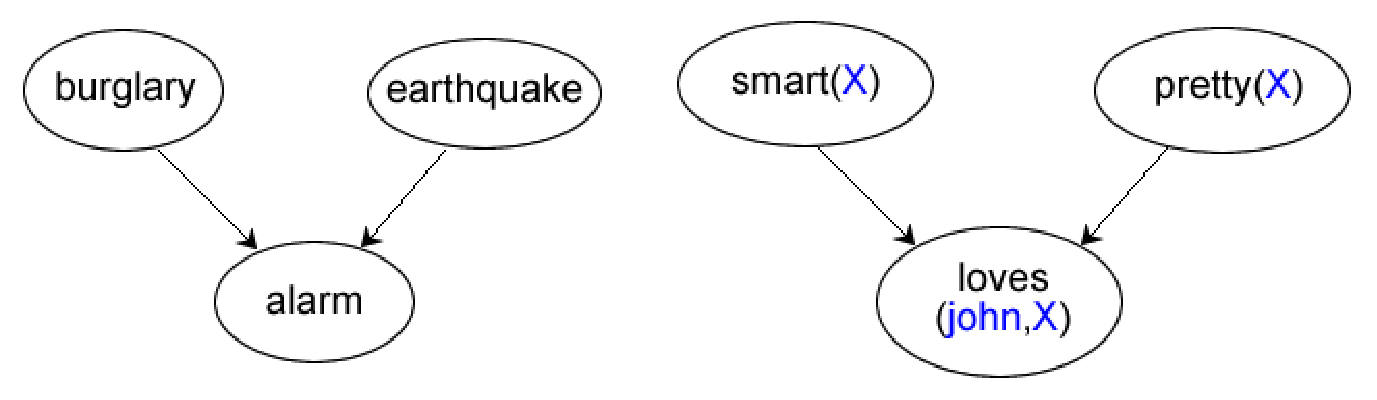
\includegraphics[scale=0.7]{FirstOrderBayesNet.eps}
\caption{propositional vs first-order Bayesian networks}
\end{figure}

One key idea in first-order Bayesian networks is the method of Knowledge-Based Model Construction (KBMC), first developed by \citep*{Wellman1992} and \citep*{Haddawy1994}.  The idea is to store a knowledgebase of first-order rules that can be used to construct propositional Bayesian networks on demand.  When a query is asked, a Bayesian network is generated on-the-fly to answer the query.  This idea helps us think of the first-order case in terms of the propositional case (though it may not be the most efficient implementation in practice).

Also, I have chosen the ``directed'' approach based on Bayesian networks, versus the ``undirected'' approach based on Markov networks (eg \citep*{Domingos2007}'s Markov Logic Network (MLN)).  It seems that the directed approach is more intuitive, in which probabilistic conditionals are used to represent \emph{causal} relations.

See the book \citep*{Getoor2007} for a collection of first-order probabilistic logic approaches.

{\bfseries Some first-order probabilistic logics:}

\citep*{Kersting2000}'s Bayesian Logic Program (BLP)

\citep*{Laskey2006}'s Multi-Entity Bayesian Network (MEBN)

\citep*{Getoor2007a}'s Probabilistic Relational Model (PRM)

\citep*{Milch2007}'s Bayesian Logic (BLOG)

{\bfseries Other first-order probabilistic logics I have not looked into:}

\citep*{Sato1997}'s PRISM

\citep*{Muggleton1996}'s Stochastic Logic Program (SLP)

\citep*{Jaeger1997}'s Relational Bayesian Network (RBN), etc...

\subsection{Bayesian networks and classical logic}
\label{sec:P-and-ClassicalLogic}

Now we examine the relation between Bayesian networks and classical logic.

\textbf{The problem with ``material implication''.}  The notion of implication in classical logic is no longer applicable in a probabilistic setting.  To see why, consider the classical equivalence of implication\\
\hspace*{1cm} $ A \rightarrow B \equiv \neg A \vee B $\\
and if we try to calculate the probability truth value of this statement we get\\
\hspace*{1cm} $ p = P( \neg A \vee B ) = P(\neg A) + P(B) - P(B|\neg A) P(\neg A) $\\
\hspace*{1cm} = $ 1 - P(A) + P(B|A) P(A) $\\
using 3 basic rules of probabilities:\\
\hspace*{1cm} $ P(X \vee Y) \equiv P(X) + P(Y) - P(X \wedge Y) $  (regardless of whether X,Y are independent)\\
\hspace*{1cm} $ P(X \wedge Y) \equiv P(Y|X)P(X) $\\
\hspace*{1cm} $ P(X) \equiv P(X|Y)P(Y) + P(X|\neg Y)P(\neg Y) $.

Now we have 4 things:\\
\hspace*{1cm} 1.  $ P(A) $\\
\hspace*{1cm} 2.  $ P(B) $\\ 
\hspace*{1cm} 3.  $ P(B|A) $\\
\hspace*{1cm} 4.  $ P(A \rightarrow B) = P(\neg A \vee B) = p $\\
but they cannot be fixed independently of each other: if we fix any 3 the 4th will also be fixed.

What is the problem here?  The classical implication ``$A \rightarrow B$'' serves a function \textit{similar} to the probabilistic conditional $P(B|A)$, but they constrain probabilities in slightly different ways, so they conflict with each other.  If we keep both copies of \#3 and \#4 in our KB, and apply machine learning to learn their truth values, the values may fail to converge.  It seems that classical implication is only \emph{accidentally} equivalent to $\neg A \vee B$ when things are binary.  In the probabilistic setting, we should jettison the binary implication in favor of the probabilistic conditional.

\textbf{Translating classical logic to Bayesian network.}  First, we can translate a first-order KB into Horn form.  This is generally impossible, since Horn logic is a strict subset of first-order logic, but it can be done if we compile the knowledgebase into a pseudo-Horn form and use a special inference algorithm (this is done in \citep*{Stickel1988}).  A Horn formula (which is equivalent to a Prolog statement) having the form:\\
\hspace*{1cm} \ttfamily A :- B, C, D, ... \rmfamily\\
would corresponds to:\\
\hspace*{1cm} $ P(A | B, C, D, ...) = p $\\
in a Bayesian network.  This approach is also adopted by BLP, MEBN, BLOG, and PRM (see \S\ref{sec:FOL-BN}).

\subsection{Interval-valued probabilities}
\label{sec:intervalP}

Sometimes, Bayesian networks fail to reproduce analogous results in classical logic unless we use interval probabilities.  Consider this example:
\begin{quote}
\emph{China and the US are in conflict. If John sides with the US, he'll be a traitor. If he sides with China, he'll be a loser. Either way, John will be miserable.}
\end{quote}

We can express the premises as conditional probabilities:\\
\hspace*{1cm} $P(\mbox{miserable} \,|\, \mbox{traitor} ) = 0.9$ \\
\hspace*{1cm} $P(\mbox{miserable} \,|\, \neg\mbox{traitor} ) = 0.8$ \\
and we want to query the probability $P(\mbox{miserable})$, but it is unknown whether John is a traitor or a patriot.

This example is exactly analogous to the ``resolution rule'' in classical logic.  The classical inference step is:

\hspace*{1cm} traitor $\rightarrow$ miserable\\
\hspace*{1cm} $\neg$ traitor $\rightarrow$ miserable\\ 
\hspace*{1cm} --------------------------------\\
\hspace*{1cm} miserable

If we construct a Bayesian network we will have the following CPT (conditional probability table):\\
\hspace*{1cm} \begin{tabular}{|l|l|} \hline
\textbf{traitor} & \textbf{miserable}\\ \hline
true             & 0.9\\
false            & 0.8\\ \hline
\end{tabular}

but we cannot evaluate $P(\mbox{miserable})$ since $P(\mbox{traitor})$ is not known.  This is a problem with point-valued Bayesian networks: \emph{they fail to draw some analogous conclusions of classical logic}.

However, according to probability theory:\\
\hspace*{1cm} $ P(A) = P(A | B) P(B) + P(A | \neg B) P(\neg B) $

Therefore:\\
\hspace*{1cm} $ P(\mbox{miserable}) = P(\mbox{miserable} \,|\, \mbox{traitor}) P(\mbox{traitor}) + P(\mbox{miserable} \,|\, \neg\mbox{traitor}) P(\neg\mbox{traitor}) $\\
\hspace*{1cm} $= 0.9 P(\mbox{traitor}) + 0.8 P(\neg\mbox{traitor}) $\\
\hspace*{1cm} $= 0.9 p + 0.8 (1 - p) $\\ 
\hspace*{1cm} $= 0.8 + 0.1 p $\\
\hspace*{1cm} $= [0.8, 0.9] $

In other words, if we allow the use of interval probability, we can infer that $P(\mbox{miserable}) = [0.8, 0.9]$ even when we assume that $P(\mbox{traitor}) = [0,1]$ (ie, unknown). Thus we obtain a result analogous to classical resolution.

We need a Bayesian network inference algorithm that can handle this type of deduction, but first we consider an important simplification in the next section.  The final algorithm will be given in \S\ref{sec:P-inference}.

\subsection{Why point-valued probability is sufficient for AGI}
\label{sec:PointValued}

In my opinion, second-order probability (such as interval probability or the indefinite probability developed by \citep*{Walley1991} and used in \citep*{Goertzel2008}) is an overkill for AGI.  It makes the deduction algorithm very complex, and since the machine learning algorithm is based on deduction and is \textit{even more} complex, the latter problem becomes practically impossible to solve in those settings.  So we must make the deduction algorithm as simple as possible.  Therefore I suggest using only point-valued probability.

In \S\ref{sec:intervalP} I showed that interval probability is needed for some inference steps.  That means the probability P itself is uncertain, and it lies in an interval.  The \emph{exact} algorithm for interval-probability inference requires us to set up the bounds of various probabilities and then invoke linear programming to solve for the probability bounds of the query variable (This method was first outlined by \citep*{Boole1854} and then developed by \citep*{Hailperin1965}, \citep*{Nilsson1986}, \citep*{Ng1992} et al. Recently \citep*{Hansen2000}, \citep*{Jaumard2006} developed faster algorithms for it, but still, the complexity of these algorithms is too much to handle if we want to design learning algorithms based on them.)

What I propose is that whenever we obtain an interval P value, we should convert it to a point value by \emph{taking the mid-point of the interval}.\footnote{We still need inference algorithms that can handle intervals as demonstrated in \S\ref{sec:intervalP}, but the intervals will be instantly converted to point-values after each step. This reduces complexity greatly.}

For example, John may be unable to decide whether the president is smart or dumb.  He may ascribe $P = [0.2,0.8]$ to the atom $smart(president)$.  According to my scheme, he can use \[ P = (0.2 + 0.8) / 2 = 0.5 \] as a compromise.  This is like saying ``there's 50-50 chance''.  Is this approximation too bad?  It seems that many people think like this anyway.  I'd be surprised if the human brain maintains 2nd-order probabilities internally.

Moreover, the exact values of P often do not affect our behavior that much.  There is evidence that taking the centroid (the center of mass of a belief distribution) can yield reasonably good results in second-order probabilistic decision-making (\citep*{Sundgren2006}).  Also, \citep*{Bier1993} shows that there are broad classes of utility functions for which uncertainty is irrelevant under expected utility theory, and only mean values are significant.  \{ TODO:  There is hand-waving here. \}

Maybe in a much more advanced AGI, we would want 2nd-order precision, but that seems not to be the right priority now.  It may be more effective for an AGI to improve its decisions by:\\
\hspace*{1cm} 1. considering more factors;\\
\hspace*{1cm} 2. updating probabilities using more evidence;\\
\hspace*{1cm} 3. refining explanations (causal relations);  etc.

Using point-valued probabilities (without knowing their error) is not such a big sin, if we compare this with what we do in fuzzy logic all the time.  A fuzzy statement such as:\\
\hspace*{1cm} ``John is fairly tall''\\
is often represented simply by:\\
\hspace*{1cm} tall(john) \hspace{0.5cm} $z = 0.7$\\
which is analogous to representing the probabilistic statement\\
\hspace*{1cm} ``John is usually punctual''\\
with a point-valued probability:\\
\hspace*{1cm} punctual(john) \hspace{0.5cm} $p = 0.8$.

If fuzziness is a more fundamental phenomenon in our knowledge representation, we should be making more fuss about fuzziness than probabilities.  It seems that we ascribe more ``prestige'' to probability theory merely because of psychological reasons.

\subsection{Probabilistic AND and OR}
\label{sec:probabilistic-AND-OR}

Specifying the CPT (conditional probability table) of a single node of a Bayesian network, if the node has $n$ parents, would require $2^n$ entries.  The ``noisy'' AND and OR gates are designed to simplify this by reducing the number of independent entries to $n$.  The interpretation of the noisy OR gate is that each parent variable $X$ is associated with an ``inhibition probability'', $q$ (\citep*{Pearl1988} p184-187 or \citep*{Russell2003} p500-501).  This is the textbook definition of noisy OR (and I created noisy AND by applying DeMorgan's laws\footnote{That is, to require $\overline{X_1 \curlyvee X_2} \equiv \overline{X_1} \curlywedge \overline{X_2}$ and $\overline{X_1 \curlywedge X_2} \equiv \overline{X_1} \curlyvee \overline{X_2}$ }):

\hspace*{1cm} \begin{tabular}{|l|l||l||l|} \hline
\multicolumn{2}{|c||}{} & {\textbf{noisy AND}}           & {\textbf{noisy OR}}\\ \hline
$X_1$ & $X_2$           & $X_1 \curlywedge X_2$          & $ X_1 \curlyvee X_2 $\\ \hline
0     & 0               & $ 1 ? $                        & $ 0 $\\
0     & 1               & $ 1 - q_1 ? $                  & $ 1 - q_1 $\\
1     & 0               & $ 1 - q_2 ? $                  & $ 1 - q_2 $\\
1     & 1               & $ 1 - q_1 - q_2 + q_1 q_2 ? $  & $ 1 - q_1 q_2 $\\ \hline
\end{tabular}

It seem that this definition of noisy AND is problematic (for example, the ``1'' should be close to 0).

So, I define my version of ``probabilistic'' AND and OR via DeMorgan's laws.  Each variable is attached with a ``causal strength'' $c \in [0,1]$, such that when $c \rightarrow 1$ they reduce to classical AND and OR.  (Unfortunately, the original ``noisy-OR'' interpretation is lost.)

\hspace*{1cm} \begin{tabular}{|l|l||l||l|}
\hline
\multicolumn{2}{|c||}{} & {\textbf{probabilistic AND}} & {\textbf{probabilistic OR}}\\
\hline
%\rule[-3mm]{0mm}{8mm}
$X_1$ & $X_2$ & $X_1 \curlywedge X_2$          & $X_1 \curlyvee X_2$\\ \hline
0     & 0     & $(1-c_1) (1-c_2)$              & $1 - c_1 c_2$\\
0     & 1     & $(1-c_1) \; c_2$               & $1 - c_1 + c_1 c_2$\\
1     & 0     & $c_1 \; (1-c_2)$               & $1 - c_2 + c_1 c_2$\\
1     & 1     & $c_1 \; c_2$                   & $c_1 + c_2 - c_1 c_2$\\
\hline
\end{tabular}
\parbox{5cm}{\begin{equation}
\label{eqn:probabilistic-AND-OR}
\end{equation}}

This can be easily generalized to $n > 2$.

A CPT can be defined by a combination of probabilistic AND-OR's:
\begin{equation}
X_0 := \bigcurlyvee_i \; \bigcurlywedge_j \; X_{ij}
\end{equation}
where the $X_{ij}$'s are parents of the node $X_0$ in the Bayesian network.

Notice that in the above equation, each connective is associated with a pair of c parameters, so the actual equation is:
\begin{equation}
X_0 := \bigcurlyvee_i \; \bigcurlywedge_j \; X_{ij};c_{ij} \; = \bigcurlyvee \; \{ X_{11};c_{11} \curlywedge X_{12};c_{12} \curlywedge \cdots, X_{21};c_{21} \curlywedge X_{22};c_{22} \curlywedge \cdots, \; \cdots \}
\end{equation}
And, because of the c parameters, commutation does not hold in general, ie: $((A \curlyvee B) \curlyvee C) \neq (A \curlyvee (B \curlyvee C))$.

% TO-DO:  weighted noisy AND-OR may not be needed, because the weights are absorbed into the c's

\subsection{P inference algorithm}
\label{sec:P-inference}

The $\mathcal{P}$ inference algorithm is similar to $\mathcal{Z}$ inference (Algorithm \ref{algorithm1}) except that probabilistic inference can be ``abductive'' --- a conditional probability can work in the reverse direction via Bayes theorem --- thus the branching factor of the search would be higher.

\begin{algorithm}
\caption{backward-chaining P inference}
\label{algorithm2}
\begin{algorithmic}[1]

\REQUIRE a knowledgebase $KB$, a list of query goals $G$ \\
\ENSURE $p =$ probability of $G$.

\REPEAT
	\STATE choose a literal $L$ from the list $G$, removing it from G
	\STATE find a rule $X_0 \leftarrow \bigcurlyvee \bigcurlywedge X_{ij} $ such that\\
			 $L$ unifies with one of the $X_{ij}$'s, including $X_0$\\
	\COMMENT{ if $X_{ij}$ is null, $X_0$ is a fact in $KB$ }
	\STATE add the $X$'s to the list $G$, except the one that unifies with $L$ \\
	\STATE if depth of recursion $< h$ \\
			 recurse to resolve the new list of goals $G$ \\
\UNTIL{ there are no more applicable rules in $KB$. }

\end{algorithmic}
\end{algorithm}

TO-DO: Deal with loops.

TO-DO: There should be a mechanism to prune low-probability branches early on in the search.

TO-DO: Compare $\mathcal{P}$ inference with standard Bayesian network inference algorithms...?\\
This algorithm merely outlines the rules involved in computing $P(X)$.

Problems of Bayesian network inference:\\
1.  Some inference steps analogous to classical logic cannot be performed because probabilities are not truth-functional (ie, the probability of a statement is not the function of the probabilities of its constituents; it may depend on other probabilities not appearing in the statement).\\
2.  Bayesian network inference cannot be performed one-rule-per-step because of interdependence of variables that require message passing.

The solution to \#1 is to use 0.5 as the substitute for unknown probabilities.

The solution to \#2 is to use only local dependencies.

Case \#1:
\begin{figure}[H]
\centering
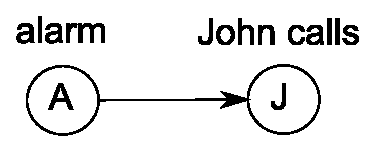
\includegraphics{BayesNet-alarm-John.eps}
\end{figure}
\textbf{Forward inference}: the answer is simply what is given: $P(J|A)$\\
\textbf{Backward inference (abduction)}: we seek $P(A|J)$ which is given by Bayes rule:\\
$$ P(A|J) = \frac{P(J|A)P(A)}{P(J)} $$
and we search for values of $P(A)$ and $P(J)$; If they don't exist we substitute with 0.5.

It seems that we need to record the rule during inference.  When the subgoals are all found we can obtain the head.  Is there a way not to store the rules?  No.  Not only that, but we need to have backtrack ability too.

Case \#2:
\begin{figure}[H]
\centering
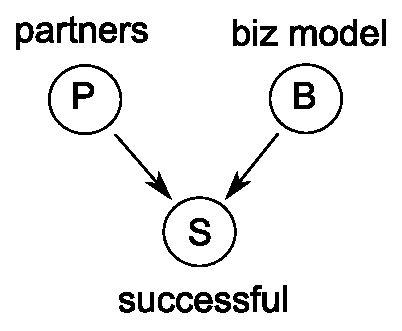
\includegraphics{BayesNet-successful-business.eps}
\end{figure}
\textbf{Forward inference}: simply given by $P(S|P,B)$\\
\textbf{Abduction}: given S, we can infer P and B.  "P or B" is a problem. How to represent that?  

\section{Combining B, P, Z}
\label{sec:combinePZ}

\subsection{The truth value P(Z)}

How to combine $\mathcal{P}$ and $\mathcal{Z}$?  The answer is simple because there is no other choice:  the semantics of probabilities dictate that $\mathcal{P}$ must be \textit{distributed over events}.  In our AGI, events are either $\mathcal{B}$ or $\mathcal{Z}$ (the latter as \textit{continuous} events).  So we \emph{distribute $\mathcal{P}$ over $\mathcal{B}$ and $\mathcal{Z}$}.  In this sense, fuzziness is more fundamental than probabilities.

If a $\mathcal{Z}$ value is uncertain --- for example, we may not be sure how tall Mary is (the $\mathcal{Z}$-value of her tallness may be 0.6-0.8, say, so we can assume a uniform probability distribution over the interval [0.6,0.8] which is the green rectangle below) --- and we can approximate it by a Beta distribution over $\mathcal{Z}$ with a mean at 0.7 and the same variance:
\begin{figure}[H]
\centering
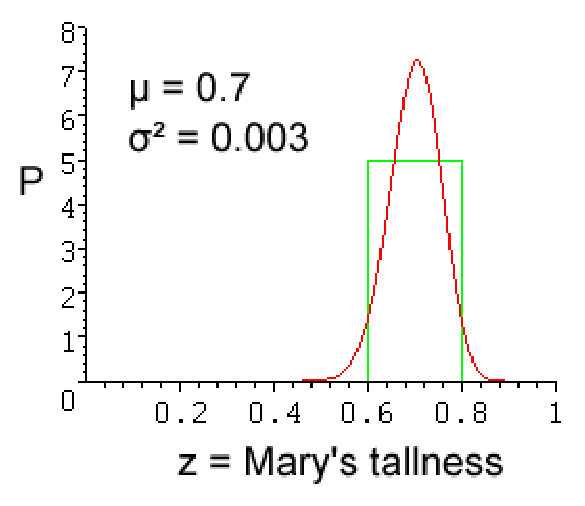
\includegraphics[scale=0.7]{P-over-Z-Marys-Tallness2.eps}
\caption{an example $\mathcal{P}(\mathcal{Z})$ distribution}
\end{figure}
where the probability density should sum to 1: $ \int^1_0 P(z) dz = 1 $.

On the other hand, if a $\mathcal{P}$ value is uncertain, we simply \textit{ignore} its error (eg, by choosing the mid-point of a P-interval).  \S\ref{sec:PointValued} tried to justify this.

\subsection{Unifying all truth values as P(Z)}

\textbf{Binary variables.}  Some variables have a strong ``binary flavor''.  For example, in common sense, a person is either dead or alive, although a more nuanced view will have grades of being dead.  If deadness is a $\mathcal{Z}$ variable, z = 0 would be ``definitely alive'', z = 1 would be ``definitely dead'' (eg reduced to ash), and z = 0.5 would correspond to a state that is difficult to classify as dead or alive, eg a brain-dead, vegetative state.  z = 0.7 may be a state that is more dead than brain-dead and yet more alive than ash --- I have to pause for a while to think of an example: a body under cryonic preservation.  And z = 0.2 may be a state of hallucination.  Anyway, one can expect the probability distribution of $z_{dead}$ to be polarized with a trough in the middle.  This can be represented by a Beta distribution with a large variance:
\begin{figure}[H]
\centering
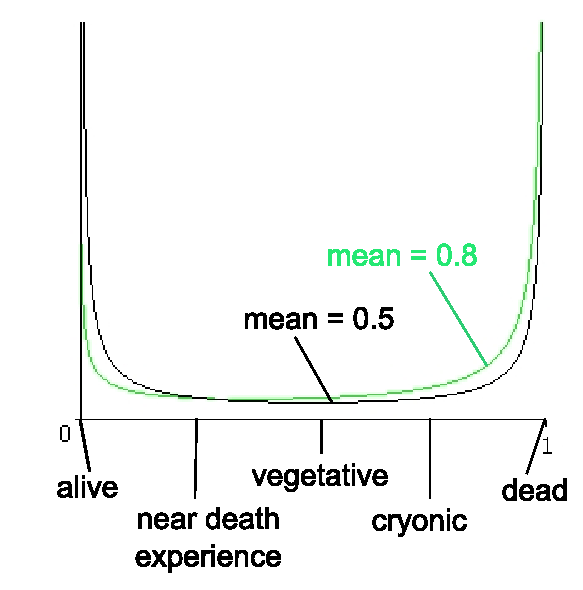
\includegraphics[scale=0.7]{deadness.eps}
%\caption{Z = deadness}
\end{figure}
The amount of variance (ie degree of polarization) can be estimated statistically, or one can use some typical values if one is reckless.

My observation is that all common-sensical ``binary'' variables are actually \textbf{polarized} $\mathcal{Z}$ variables.  Another example is a person being either married or not married, but there are grey areas like gay marriage or marriage for the green card, etc.

This can be rather arbitrary.  Also, once we established that a variable is polarized, what if we then assert its probability?  Eg P(dead) = 0.7?  This is interesting.

Equally interesting, is when we know P(dead) = 0.7, and then assert its polarity.

\subsection{Hybrid B-P-Z inference}

There are 4 possible types of truth values (TVs):

\begin{table}[H]
\parbox{3cm}{\caption{}}
\begin{tabular}{|l|l|l|} \hline
\multicolumn{3}{|c|}{\textbf{truth values}}\\ \hline
mnemonic                   & meaning                                      & definition \\ \hline
$\mathcal{B}$              & binary                                       & $b \in \{true, false\} $\\
$\mathcal{Z}$              & fuzzy                                        & $z \in [0,1] $\\
$\mathcal{P}(\mathcal{B})$ & $\mathcal{P}$ distributed over $\mathcal{Z}$ & $ P(b=false) = p_0 $\\
                           &                                              & $ P(b=true) = p_1 $\\
$\mathcal{P}(\mathcal{Z})$ & $\mathcal{P}$ distributed over $\mathcal{Z}$ & $ P(z=z_1) \sim Beta(z_1) $\\ \hline
\end{tabular}
\end{table}

Rules, which are the building blocks of inference, can be of 3 types:

\begin{table}[H]
\parbox{3cm}{\caption{}}
\begin{tabular}{|l|l|} \hline
\multicolumn{2}{|c|}{\textbf{rules}}\\ \hline
mnemonic                   & meaning\\ \hline
$\mathcal{B}$              & Prolog statements of the form\\
                           & \qquad $L_0 \, \mbox{:--} \, L_1, L_2, L_3, ... $ \\
$\mathcal{Z}$              & Fuzzy rules of the form\\
                           & \qquad $z_0 := \widetilde{\bigvee} \; \widetilde{\bigwedge} \; z_{ij}$ \\
$\mathcal{P}(\mathcal{B})$ & Bayesian network nodes specified by\\
                           & \qquad $X_0 := \bigcurlyvee \bigcurlywedge X_{ij};c_{ij}$ \\
\hline
\end{tabular}
\end{table}

giving rise to $4 \times 3 = 12$ combinations when we try to ``plug'' variables into rules:

\begin{table}[H]
\parbox{3cm}{\caption{\label{table:TV-rules-combinations}}}
\begin{tabular}{|l||l|l|l|} \hline
                           & \multicolumn{3}{c|}{\textbf{rule}}\\ \hline
\textbf{variables}         & $\mathcal{B}$ & $\mathcal{Z}$ & $\mathcal{P}(\mathcal{B})$ \\ \hline
$\mathcal{B}$              & case 1        & case 5        & case 9  \\
$\mathcal{Z}$              & case 2        & case 6        & case 10 \\
$\mathcal{P}(\mathcal{B})$ & case 3        & case 7        & case 11 \\
$\mathcal{P}(\mathcal{Z})$ & case 4        & case 8        & case 12 \\ \hline
\end{tabular}
\end{table}

The TV type of a rule is determined by its ``head'' --- eg, if the head is a $\mathcal{B}$ variable then the rule is a $\mathcal{B}$-rule.  A rule may involve factors of TV types other than its own TV type, which is handled by Table \ref{table:TV-rules-combinations}.

For example, ``almost Q'' means ``close to Q, but not being Q'', which translates to this rule:\\
\hspace*{1cm} $\mbox{almost } Q \leftarrow \mbox{ close-to } Q \wedge \neg Q$\\
where the head is of type $\mathcal{B}$, the first factor is of type $\mathcal{Z}$, the second factor is of type $\mathcal{B}$.

%In general, inference proceeds by drawing rules from the KB.  Conclusions of various TV types will be generated depending on the TV type of the rules being applied.

To simplify things, I consider single inference steps.  A complete proof involves a series of such steps.

An essential trick is that truth value types can be inter-converted:
\begin{figure}[H]
\centering
%LaTeX with PSTricks extensions
%%Creator: 0.46
%%Please note this file requires PSTricks extensions
\psset{xunit=.5pt,yunit=.5pt,runit=.5pt}
\begin{pspicture}(205.73828125,167.16601562)
{
\newrgbcolor{curcolor}{0 0 0}
\pscustom[linestyle=none,fillstyle=solid,fillcolor=curcolor]
{
\newpath
\moveto(27.08398812,133.22851301)
\lineto(27.08398812,148.97655988)
\lineto(32.99219125,148.97655988)
\curveto(34.19530753,148.97654413)(35.16031307,148.81720185)(35.88721078,148.49853254)
\curveto(36.61408766,148.17983269)(37.18342303,147.68927329)(37.59521859,147.02685285)
\curveto(38.00698991,146.36440482)(38.21288163,145.67153442)(38.21289437,144.94823957)
\curveto(38.21288163,144.27505144)(38.03026463,143.64126301)(37.66504281,143.04687238)
\curveto(37.29979661,142.45246212)(36.74836487,141.97264489)(36.01074594,141.60741926)
\curveto(36.96320841,141.32811428)(37.69546679,140.85187778)(38.20752328,140.17870832)
\curveto(38.71955431,139.50552496)(38.97557618,138.71060388)(38.97558969,137.7939427)
\curveto(38.97557618,137.05630866)(38.81981462,136.37059971)(38.50830453,135.73681379)
\curveto(38.19676837,135.10302285)(37.81184037,134.61425381)(37.35351937,134.2705052)
\curveto(36.89517462,133.9267545)(36.32046816,133.66715189)(35.62939828,133.4916966)
\curveto(34.93830809,133.31624078)(34.09146649,133.22851301)(33.08887094,133.22851301)
\lineto(27.08398812,133.22851301)
\closepath
\moveto(29.1679725,142.35937238)
\lineto(32.57324594,142.35937238)
\curveto(33.49706604,142.35936325)(34.15950027,142.42023559)(34.56055062,142.54198957)
\curveto(35.09048892,142.69953218)(35.48973983,142.96092515)(35.75830453,143.32616926)
\curveto(36.02684866,143.69139317)(36.16112587,144.14972604)(36.16113656,144.70116926)
\curveto(36.16112587,145.22394372)(36.03580048,145.68406696)(35.78516,146.08154035)
\curveto(35.5344989,146.47898804)(35.17642634,146.75112318)(34.71094125,146.8979466)
\curveto(34.24543769,147.04474268)(33.44693588,147.11814756)(32.31543344,147.11816145)
\lineto(29.1679725,147.11816145)
\lineto(29.1679725,142.35937238)
\closepath
\moveto(29.1679725,135.08691145)
\lineto(33.08887094,135.08691145)
\curveto(33.76203973,135.08690959)(34.23469551,135.11197467)(34.50683969,135.16210676)
\curveto(34.98664788,135.24804224)(35.38768915,135.39127126)(35.70996469,135.59179426)
\curveto(36.03221975,135.79231253)(36.29719345,136.08414166)(36.50488656,136.46728254)
\curveto(36.71255761,136.85041694)(36.81639866,137.29263655)(36.81641,137.7939427)
\curveto(36.81639866,138.38117713)(36.66600818,138.89143052)(36.36523812,139.32470441)
\curveto(36.06444628,139.75796611)(35.64729175,140.06232779)(35.11377328,140.23779035)
\curveto(34.58023553,140.4132389)(33.81216989,140.50096667)(32.80957406,140.50097395)
\lineto(29.1679725,140.50097395)
\lineto(29.1679725,135.08691145)
\closepath
}
}
{
\newrgbcolor{curcolor}{0 0 0}
\pscustom[linestyle=none,fillstyle=solid,fillcolor=curcolor]
{
\newpath
\moveto(166.91308969,129.22851301)
\lineto(166.91308969,131.16210676)
\lineto(174.9804725,141.24902082)
\curveto(175.55338009,141.96515392)(176.09765037,142.58820017)(176.613285,143.11816145)
\lineto(167.82617562,143.11816145)
\lineto(167.82617562,144.97655988)
\lineto(179.1054725,144.97655988)
\lineto(179.1054725,143.11816145)
\lineto(170.26465219,132.19335676)
\lineto(169.3085975,131.08691145)
\lineto(179.363285,131.08691145)
\lineto(179.363285,129.22851301)
\lineto(166.91308969,129.22851301)
\closepath
}
}
{
\newrgbcolor{curcolor}{0 0 0}
\pscustom[linestyle=none,fillstyle=solid,fillcolor=curcolor]
{
\newpath
\moveto(11.16992562,19.22851301)
\lineto(11.16992562,34.97655988)
\lineto(17.11035531,34.97655988)
\curveto(18.15591955,34.97654413)(18.95442135,34.92641398)(19.50586312,34.82616926)
\curveto(20.27928982,34.69724754)(20.92740115,34.45196784)(21.45019906,34.09032941)
\curveto(21.97297302,33.72866127)(22.39370828,33.2219886)(22.71240609,32.57030988)
\curveto(23.03107743,31.91860448)(23.19041972,31.20245937)(23.19043344,30.42187238)
\curveto(23.19041972,29.08266982)(22.76431338,27.94937017)(21.91211312,27.02197004)
\curveto(21.059888,26.09455432)(19.52017599,25.63085036)(17.2929725,25.63085676)
\lineto(13.25391,25.63085676)
\lineto(13.25391,19.22851301)
\lineto(11.16992562,19.22851301)
\closepath
\moveto(13.25391,27.4892552)
\lineto(17.32519906,27.4892552)
\curveto(18.67154403,27.48924693)(19.62759776,27.73989773)(20.19336312,28.24120832)
\curveto(20.75910705,28.74250089)(21.04198437,29.44790383)(21.04199594,30.35741926)
\curveto(21.04198437,31.01626164)(20.87548063,31.58022592)(20.54248422,32.04931379)
\curveto(20.20946567,32.51837602)(19.77082679,32.82810878)(19.22656625,32.97851301)
\curveto(18.87564539,33.07159812)(18.22753406,33.11814756)(17.28223031,33.11816145)
\lineto(13.25391,33.11816145)
\lineto(13.25391,27.4892552)
\closepath
}
}
{
\newrgbcolor{curcolor}{0 0 0}
\pscustom[linestyle=none,fillstyle=solid,fillcolor=curcolor]
{
\newpath
\moveto(29.31348031,14.5986302)
\curveto(28.24641894,15.94498765)(27.34407609,17.5205069)(26.60644906,19.3251927)
\curveto(25.86881715,21.12987829)(25.50000242,22.99901705)(25.50000375,24.93261457)
\curveto(25.50000242,26.63703425)(25.77571829,28.26984511)(26.32715219,29.83105207)
\curveto(26.97168063,31.64288861)(27.96712235,33.44757431)(29.31348031,35.24511457)
\lineto(30.6992225,35.24511457)
\curveto(29.83268038,33.75551671)(29.25976428,32.69204121)(28.9804725,32.05468488)
\curveto(28.54361917,31.06639179)(28.19986951,30.03514283)(27.9492225,28.96093488)
\curveto(27.64127632,27.62173378)(27.48730512,26.27538096)(27.48730844,24.92187238)
\curveto(27.48730512,21.47720868)(28.55794207,18.03613139)(30.6992225,14.5986302)
\lineto(29.31348031,14.5986302)
\closepath
}
}
{
\newrgbcolor{curcolor}{0 0 0}
\pscustom[linestyle=none,fillstyle=solid,fillcolor=curcolor]
{
\newpath
\moveto(33.12695687,19.22851301)
\lineto(33.12695687,34.97655988)
\lineto(39.03516,34.97655988)
\curveto(40.23827628,34.97654413)(41.20328182,34.81720185)(41.93017953,34.49853254)
\curveto(42.65705641,34.17983269)(43.22639178,33.68927329)(43.63818734,33.02685285)
\curveto(44.04995866,32.36440482)(44.25585038,31.67153442)(44.25586312,30.94823957)
\curveto(44.25585038,30.27505144)(44.07323338,29.64126301)(43.70801156,29.04687238)
\curveto(43.34276536,28.45246212)(42.79133362,27.97264489)(42.05371469,27.60741926)
\curveto(43.00617716,27.32811428)(43.73843554,26.85187778)(44.25049203,26.17870832)
\curveto(44.76252306,25.50552496)(45.01854493,24.71060388)(45.01855844,23.7939427)
\curveto(45.01854493,23.05630866)(44.86278337,22.37059971)(44.55127328,21.73681379)
\curveto(44.23973712,21.10302285)(43.85480912,20.61425381)(43.39648812,20.2705052)
\curveto(42.93814337,19.9267545)(42.36343691,19.66715189)(41.67236703,19.4916966)
\curveto(40.98127684,19.31624078)(40.13443524,19.22851301)(39.13183969,19.22851301)
\lineto(33.12695687,19.22851301)
\closepath
\moveto(35.21094125,28.35937238)
\lineto(38.61621469,28.35937238)
\curveto(39.54003479,28.35936325)(40.20246902,28.42023559)(40.60351937,28.54198957)
\curveto(41.13345767,28.69953218)(41.53270858,28.96092515)(41.80127328,29.32616926)
\curveto(42.06981741,29.69139317)(42.20409462,30.14972604)(42.20410531,30.70116926)
\curveto(42.20409462,31.22394372)(42.07876923,31.68406696)(41.82812875,32.08154035)
\curveto(41.57746765,32.47898804)(41.21939509,32.75112318)(40.75391,32.8979466)
\curveto(40.28840644,33.04474268)(39.48990463,33.11814756)(38.35840219,33.11816145)
\lineto(35.21094125,33.11816145)
\lineto(35.21094125,28.35937238)
\closepath
\moveto(35.21094125,21.08691145)
\lineto(39.13183969,21.08691145)
\curveto(39.80500848,21.08690959)(40.27766426,21.11197467)(40.54980844,21.16210676)
\curveto(41.02961663,21.24804224)(41.4306579,21.39127126)(41.75293344,21.59179426)
\curveto(42.0751885,21.79231253)(42.3401622,22.08414166)(42.54785531,22.46728254)
\curveto(42.75552636,22.85041694)(42.85936741,23.29263655)(42.85937875,23.7939427)
\curveto(42.85936741,24.38117713)(42.70897693,24.89143052)(42.40820687,25.32470441)
\curveto(42.10741503,25.75796611)(41.6902605,26.06232779)(41.15674203,26.23779035)
\curveto(40.62320428,26.4132389)(39.85513864,26.50096667)(38.85254281,26.50097395)
\lineto(35.21094125,26.50097395)
\lineto(35.21094125,21.08691145)
\closepath
}
}
{
\newrgbcolor{curcolor}{0 0 0}
\pscustom[linestyle=none,fillstyle=solid,fillcolor=curcolor]
{
\newpath
\moveto(48.92871469,14.5986302)
\lineto(47.5429725,14.5986302)
\curveto(49.68424507,18.03613139)(50.75488202,21.47720868)(50.75488656,24.92187238)
\curveto(50.75488202,26.26821951)(50.60091082,27.60383015)(50.2929725,28.92870832)
\curveto(50.04947908,30.0029163)(49.70931015,31.03416526)(49.27246469,32.02245832)
\curveto(48.99316503,32.66697613)(48.41666821,33.74119381)(47.5429725,35.24511457)
\lineto(48.92871469,35.24511457)
\curveto(50.27506479,33.44757431)(51.2705065,31.64288861)(51.91504281,29.83105207)
\curveto(52.46646885,28.26984511)(52.74218472,26.63703425)(52.74219125,24.93261457)
\curveto(52.74218472,22.99901705)(52.37157962,21.12987829)(51.63037484,19.3251927)
\curveto(50.88915923,17.5205069)(49.98860674,15.94498765)(48.92871469,14.5986302)
\lineto(48.92871469,14.5986302)
\closepath
}
}
{
\newrgbcolor{curcolor}{0 0 0}
\pscustom[linestyle=none,fillstyle=solid,fillcolor=curcolor]
{
\newpath
\moveto(165.16992562,18.22851301)
\lineto(165.16992562,33.97655988)
\lineto(171.11035531,33.97655988)
\curveto(172.15591955,33.97654413)(172.95442135,33.92641398)(173.50586312,33.82616926)
\curveto(174.27928982,33.69724754)(174.92740115,33.45196784)(175.45019906,33.09032941)
\curveto(175.97297302,32.72866127)(176.39370828,32.2219886)(176.71240609,31.57030988)
\curveto(177.03107743,30.91860448)(177.19041972,30.20245937)(177.19043344,29.42187238)
\curveto(177.19041972,28.08266982)(176.76431338,26.94937017)(175.91211312,26.02197004)
\curveto(175.059888,25.09455432)(173.52017599,24.63085036)(171.2929725,24.63085676)
\lineto(167.25391,24.63085676)
\lineto(167.25391,18.22851301)
\lineto(165.16992562,18.22851301)
\closepath
\moveto(167.25391,26.4892552)
\lineto(171.32519906,26.4892552)
\curveto(172.67154403,26.48924693)(173.62759776,26.73989773)(174.19336312,27.24120832)
\curveto(174.75910705,27.74250089)(175.04198437,28.44790383)(175.04199594,29.35741926)
\curveto(175.04198437,30.01626164)(174.87548063,30.58022592)(174.54248422,31.04931379)
\curveto(174.20946567,31.51837602)(173.77082679,31.82810878)(173.22656625,31.97851301)
\curveto(172.87564539,32.07159812)(172.22753406,32.11814756)(171.28223031,32.11816145)
\lineto(167.25391,32.11816145)
\lineto(167.25391,26.4892552)
\closepath
}
}
{
\newrgbcolor{curcolor}{0 0 0}
\pscustom[linestyle=none,fillstyle=solid,fillcolor=curcolor]
{
\newpath
\moveto(183.31348031,13.5986302)
\curveto(182.24641894,14.94498765)(181.34407609,16.5205069)(180.60644906,18.3251927)
\curveto(179.86881715,20.12987829)(179.50000242,21.99901705)(179.50000375,23.93261457)
\curveto(179.50000242,25.63703425)(179.77571829,27.26984511)(180.32715219,28.83105207)
\curveto(180.97168063,30.64288861)(181.96712235,32.44757431)(183.31348031,34.24511457)
\lineto(184.6992225,34.24511457)
\curveto(183.83268038,32.75551671)(183.25976428,31.69204121)(182.9804725,31.05468488)
\curveto(182.54361917,30.06639179)(182.19986951,29.03514283)(181.9492225,27.96093488)
\curveto(181.64127632,26.62173378)(181.48730512,25.27538096)(181.48730844,23.92187238)
\curveto(181.48730512,20.47720868)(182.55794207,17.03613139)(184.6992225,13.5986302)
\lineto(183.31348031,13.5986302)
\closepath
}
}
{
\newrgbcolor{curcolor}{0 0 0}
\pscustom[linestyle=none,fillstyle=solid,fillcolor=curcolor]
{
\newpath
\moveto(185.95605844,18.22851301)
\lineto(185.95605844,20.16210676)
\lineto(194.02344125,30.24902082)
\curveto(194.59634884,30.96515392)(195.14061912,31.58820017)(195.65625375,32.11816145)
\lineto(186.86914437,32.11816145)
\lineto(186.86914437,33.97655988)
\lineto(198.14844125,33.97655988)
\lineto(198.14844125,32.11816145)
\lineto(189.30762094,21.19335676)
\lineto(188.35156625,20.08691145)
\lineto(198.40625375,20.08691145)
\lineto(198.40625375,18.22851301)
\lineto(185.95605844,18.22851301)
\closepath
}
}
{
\newrgbcolor{curcolor}{0 0 0}
\pscustom[linestyle=none,fillstyle=solid,fillcolor=curcolor]
{
\newpath
\moveto(201.68262094,13.5986302)
\lineto(200.29687875,13.5986302)
\curveto(202.43815132,17.03613139)(203.50878827,20.47720868)(203.50879281,23.92187238)
\curveto(203.50878827,25.26821951)(203.35481707,26.60383015)(203.04687875,27.92870832)
\curveto(202.80338533,29.0029163)(202.4632164,30.03416526)(202.02637094,31.02245832)
\curveto(201.74707128,31.66697613)(201.17057446,32.74119381)(200.29687875,34.24511457)
\lineto(201.68262094,34.24511457)
\curveto(203.02897104,32.44757431)(204.02441275,30.64288861)(204.66894906,28.83105207)
\curveto(205.2203751,27.26984511)(205.49609097,25.63703425)(205.4960975,23.93261457)
\curveto(205.49609097,21.99901705)(205.12548587,20.12987829)(204.38428109,18.3251927)
\curveto(203.64306548,16.5205069)(202.74251299,14.94498765)(201.68262094,13.5986302)
\lineto(201.68262094,13.5986302)
\closepath
}
}
{
\newrgbcolor{curcolor}{0 0 0}
\pscustom[linewidth=0.940534,linecolor=curcolor]
{
\newpath
\moveto(147.50239,146.22189563)
\lineto(62.34185,147.22948563)
}
}
{
\newrgbcolor{curcolor}{0 0 0}
\pscustom[linestyle=none,fillstyle=solid,fillcolor=curcolor]
{
\newpath
\moveto(72.34650173,142.93757037)
\lineto(61.09269491,147.22769692)
\lineto(72.44485636,151.25035658)
\curveto(70.61007802,148.81778896)(70.5807591,145.46026023)(72.34650173,142.93757037)
\closepath
}
}
{
\newrgbcolor{curcolor}{0 0 0}
\pscustom[linewidth=0.940534,linecolor=curcolor]
{
\newpath
\moveto(150.44237,17.35644563)
\lineto(65.28183,18.36403563)
}
}
{
\newrgbcolor{curcolor}{0 0 0}
\pscustom[linestyle=none,fillstyle=solid,fillcolor=curcolor]
{
\newpath
\moveto(75.28648173,14.07212037)
\lineto(64.03267491,18.36224692)
\lineto(75.38483636,22.38490658)
\curveto(73.55005802,19.95233896)(73.5207391,16.59481023)(75.28648173,14.07212037)
\closepath
}
}
{
\newrgbcolor{curcolor}{0 0 0}
\pscustom[linewidth=1,linecolor=curcolor]
{
\newpath
\moveto(24.47266,117.22851563)
\lineto(24.47266,48.22851563)
}
}
{
\newrgbcolor{curcolor}{0 0 0}
\pscustom[linestyle=none,fillstyle=solid,fillcolor=curcolor]
{
\newpath
\moveto(28.90976872,58.91896221)
\lineto(24.49027458,46.90049718)
\lineto(20.07078142,58.91896287)
\curveto(22.68004841,56.99891463)(26.24997851,57.00997799)(28.90976872,58.91896221)
\closepath
}
}
{
\newrgbcolor{curcolor}{0 0 0}
\pscustom[linewidth=1,linecolor=curcolor]
{
\newpath
\moveto(181.45504,115.14252563)
\lineto(181.45504,46.14252563)
}
}
{
\newrgbcolor{curcolor}{0 0 0}
\pscustom[linestyle=none,fillstyle=solid,fillcolor=curcolor]
{
\newpath
\moveto(185.89214872,56.83297221)
\lineto(181.47265458,44.81450718)
\lineto(177.05316142,56.83297287)
\curveto(179.66242841,54.91292463)(183.23235851,54.92398799)(185.89214872,56.83297221)
\closepath
}
}
{
\newrgbcolor{curcolor}{0 0 0}
\pscustom[linewidth=1,linecolor=curcolor,linestyle=dashed,dash=6 6]
{
\newpath
\moveto(65.47266,33.22851563)
\lineto(148.47266,33.22851563)
}
}
{
\newrgbcolor{curcolor}{0 0 0}
\pscustom[linestyle=none,fillstyle=solid,fillcolor=curcolor]
{
\newpath
\moveto(137.78221342,37.66562435)
\lineto(149.80067845,33.24613021)
\lineto(137.78221276,28.82663705)
\curveto(139.702261,31.43590404)(139.69119764,35.00583414)(137.78221342,37.66562435)
\closepath
}
}
{
\newrgbcolor{curcolor}{0 0 0}
\pscustom[linewidth=1,linecolor=curcolor,linestyle=dashed,dash=6 6]
{
\newpath
\moveto(164.47266,50.22851563)
\lineto(164.47266,113.22851563)
}
}
{
\newrgbcolor{curcolor}{0 0 0}
\pscustom[linestyle=none,fillstyle=solid,fillcolor=curcolor]
{
\newpath
\moveto(160.03555128,102.53806905)
\lineto(164.45504542,114.55653408)
\lineto(168.87453858,102.53806839)
\curveto(166.26527159,104.45811663)(162.69534149,104.44705327)(160.03555128,102.53806905)
\closepath
}
}
{
\newrgbcolor{curcolor}{0 0 0}
\pscustom[linewidth=1,linecolor=curcolor,linestyle=dashed,dash=6 6]
{
\newpath
\moveto(40.49028,53.31450563)
\lineto(40.49028,116.31450563)
}
}
{
\newrgbcolor{curcolor}{0 0 0}
\pscustom[linestyle=none,fillstyle=solid,fillcolor=curcolor]
{
\newpath
\moveto(36.05317128,105.62405905)
\lineto(40.47266542,117.64252408)
\lineto(44.89215858,105.62405839)
\curveto(42.28289159,107.54410663)(38.71296149,107.53304327)(36.05317128,105.62405905)
\closepath
}
}
{
\newrgbcolor{curcolor}{0 0 0}
\pscustom[linewidth=1,linecolor=curcolor,linestyle=dashed,dash=6 6]
{
\newpath
\moveto(62.55865,132.21089563)
\lineto(145.55865,132.21089563)
}
}
{
\newrgbcolor{curcolor}{0 0 0}
\pscustom[linestyle=none,fillstyle=solid,fillcolor=curcolor]
{
\newpath
\moveto(134.86820342,136.64800435)
\lineto(146.88666845,132.22851021)
\lineto(134.86820276,127.80901705)
\curveto(136.788251,130.41828404)(136.77718764,133.98821414)(134.86820342,136.64800435)
\closepath
}
}
{
\newrgbcolor{curcolor}{0 0 0}
\pscustom[linestyle=none,fillstyle=solid,fillcolor=curcolor]
{
\newpath
\moveto(101.17871469,154.22851301)
\lineto(99.59668344,154.22851301)
\lineto(99.59668344,164.3095677)
\curveto(99.21581932,163.94627673)(98.7163081,163.58299584)(98.09814828,163.21972395)
\curveto(97.47998121,162.85643407)(96.92480599,162.5839734)(96.43262094,162.40234113)
\lineto(96.43262094,163.93163801)
\curveto(97.31738372,164.34764351)(98.09082044,164.85154926)(98.75293344,165.44335676)
\curveto(99.41503787,166.03514183)(99.8837874,166.60936)(100.15918344,167.16601301)
\lineto(101.17871469,167.16601301)
\lineto(101.17871469,154.22851301)
\closepath
}
}
{
\newrgbcolor{curcolor}{0 0 0}
\pscustom[linestyle=none,fillstyle=solid,fillcolor=curcolor]
{
\newpath
\moveto(111.769535,155.3798802)
\curveto(111.18359081,154.88183267)(110.61962653,154.53027052)(110.07764047,154.3251927)
\curveto(109.53564324,154.12011468)(108.95410085,154.01757572)(108.33301156,154.01757551)
\curveto(107.30761812,154.01757572)(106.51953297,154.26806375)(105.96875375,154.76904035)
\curveto(105.41797157,155.27001587)(105.14258122,155.91015195)(105.14258187,156.68945051)
\curveto(105.14258122,157.14647884)(105.24658503,157.56395889)(105.45459359,157.94189191)
\curveto(105.66260024,158.31981751)(105.9350609,158.62303986)(106.27197641,158.85155988)
\curveto(106.60888835,159.08007066)(106.9882825,159.25292205)(107.41016,159.37011457)
\curveto(107.72070365,159.4521406)(108.18945318,159.53124208)(108.81641,159.60741926)
\curveto(110.09374815,159.75975748)(111.0341769,159.94139792)(111.63769906,160.15234113)
\curveto(111.64355129,160.36913187)(111.64648097,160.50682704)(111.64648812,160.56542707)
\curveto(111.64648097,161.20995134)(111.49706706,161.66405245)(111.19824594,161.92773176)
\curveto(110.79394276,162.28514558)(110.19335742,162.46385633)(109.39648812,162.46386457)
\curveto(108.65234334,162.46385633)(108.10302748,162.33348537)(107.74853891,162.07275129)
\curveto(107.39404382,161.81200152)(107.13183705,161.3505762)(106.96191781,160.68847395)
\lineto(105.41504281,160.89941145)
\curveto(105.55566675,161.56151349)(105.78711183,162.09618092)(106.10937875,162.50341535)
\curveto(106.43164244,162.91063323)(106.89746228,163.22410948)(107.50683969,163.44384504)
\curveto(108.11621106,163.66356217)(108.82226504,163.77342534)(109.62500375,163.77343488)
\curveto(110.42187282,163.77342534)(111.06933311,163.67967543)(111.56738656,163.49218488)
\curveto(112.06542586,163.30467581)(112.43163644,163.0688362)(112.66601937,162.78466535)
\curveto(112.90038597,162.50047739)(113.0644483,162.14159103)(113.15820687,161.7080052)
\curveto(113.21093253,161.43846674)(113.23729969,160.9521391)(113.23730844,160.24902082)
\lineto(113.23730844,158.13964582)
\curveto(113.23729969,156.66894025)(113.27099106,155.7387654)(113.33838266,155.34911848)
\curveto(113.40575656,154.95946931)(113.5390572,154.58593453)(113.738285,154.22851301)
\lineto(112.08594125,154.22851301)
\curveto(111.92187132,154.55663768)(111.81640268,154.94042636)(111.769535,155.3798802)
\lineto(111.769535,155.3798802)
\closepath
\moveto(111.63769906,158.91308332)
\curveto(111.06347374,158.67870387)(110.20214648,158.47948532)(109.05371469,158.31542707)
\curveto(108.40332015,158.22167308)(107.94335967,158.11620443)(107.67383187,157.99902082)
\curveto(107.40429771,157.88182967)(107.19629011,157.71044312)(107.04980844,157.48486066)
\curveto(106.90332165,157.2592717)(106.83007954,157.00878367)(106.83008187,156.73339582)
\curveto(106.83007954,156.31151874)(106.98974735,155.95995659)(107.30908578,155.67870832)
\curveto(107.62841858,155.39745715)(108.09570327,155.25683229)(108.71094125,155.25683332)
\curveto(109.32031142,155.25683229)(109.86230307,155.39013294)(110.33691781,155.65673566)
\curveto(110.81152087,155.92333553)(111.16015333,156.28808126)(111.38281625,156.75097395)
\curveto(111.55273106,157.10839294)(111.63769192,157.63573616)(111.63769906,158.3330052)
\lineto(111.63769906,158.91308332)
\closepath
}
}
{
\newrgbcolor{curcolor}{0 0 0}
\pscustom[linestyle=none,fillstyle=solid,fillcolor=curcolor]
{
\newpath
\moveto(100.17871469,110.22851301)
\lineto(98.59668344,110.22851301)
\lineto(98.59668344,120.3095677)
\curveto(98.21581932,119.94627673)(97.7163081,119.58299584)(97.09814828,119.21972395)
\curveto(96.47998121,118.85643407)(95.92480599,118.5839734)(95.43262094,118.40234113)
\lineto(95.43262094,119.93163801)
\curveto(96.31738372,120.34764351)(97.09082044,120.85154926)(97.75293344,121.44335676)
\curveto(98.41503787,122.03514183)(98.8837874,122.60936)(99.15918344,123.16601301)
\lineto(100.17871469,123.16601301)
\lineto(100.17871469,110.22851301)
\closepath
}
}
{
\newrgbcolor{curcolor}{0 0 0}
\pscustom[linestyle=none,fillstyle=solid,fillcolor=curcolor]
{
\newpath
\moveto(106.13769906,110.22851301)
\lineto(104.66992562,110.22851301)
\lineto(104.66992562,123.11327863)
\lineto(106.25195687,123.11327863)
\lineto(106.25195687,118.51659895)
\curveto(106.9199222,119.35448044)(107.77246041,119.77342534)(108.80957406,119.77343488)
\curveto(109.38378692,119.77342534)(109.92724341,119.6577028)(110.43994516,119.42626691)
\curveto(110.95263301,119.19481264)(111.37450759,118.86961765)(111.70557016,118.45068098)
\curveto(112.0366163,118.03172786)(112.29589338,117.52635727)(112.48340219,116.9345677)
\curveto(112.67089301,116.34276471)(112.76464292,115.70995284)(112.76465219,115.0361302)
\curveto(112.76464292,113.43651761)(112.3691355,112.20019072)(111.57812875,111.32714582)
\curveto(110.78710583,110.45409872)(109.83788803,110.01757572)(108.7304725,110.01757551)
\curveto(107.62890586,110.01757572)(106.76464892,110.4775362)(106.13769906,111.39745832)
\lineto(106.13769906,110.22851301)
\closepath
\moveto(106.12012094,114.9658177)
\curveto(106.12011831,113.84667345)(106.27246191,113.03808051)(106.57715219,112.54003645)
\curveto(107.07519548,111.72558182)(107.74902293,111.31835567)(108.59863656,111.31835676)
\curveto(109.29003701,111.31835567)(109.88769267,111.61864834)(110.39160531,112.21923566)
\curveto(110.89550416,112.81981901)(111.14745703,113.71483765)(111.14746469,114.90429426)
\curveto(111.14745703,116.12303836)(110.90575806,117.02245153)(110.42236703,117.60253645)
\curveto(109.93896215,118.18260662)(109.35449008,118.47264539)(108.66894906,118.47265363)
\curveto(107.97753833,118.47264539)(107.37988267,118.17235272)(106.87598031,117.57177473)
\curveto(106.37207118,116.97118205)(106.12011831,116.10253057)(106.12012094,114.9658177)
\lineto(106.12012094,114.9658177)
\closepath
}
}
{
\newrgbcolor{curcolor}{0 0 0}
\pscustom[linestyle=none,fillstyle=solid,fillcolor=curcolor]
{
\newpath
\moveto(8.53418344,80.74902082)
\lineto(8.53418344,79.22851301)
\lineto(0.01758187,79.22851301)
\curveto(0.00586259,79.609372)(0.06738597,79.97558257)(0.20215219,80.32714582)
\curveto(0.41894812,80.90722227)(0.76611574,81.47851076)(1.24365609,82.04101301)
\curveto(1.72119291,82.60350963)(2.41113362,83.25389961)(3.31348031,83.99218488)
\curveto(4.7138657,85.14061647)(5.66015381,86.05028353)(6.1523475,86.72118879)
\curveto(6.64452783,87.39207906)(6.89062133,88.02635577)(6.89062875,88.62402082)
\curveto(6.89062133,89.25096392)(6.66650046,89.77977199)(6.21826547,90.2104466)
\curveto(5.77001698,90.64109925)(5.18554491,90.85643107)(4.4648475,90.8564427)
\curveto(3.70312452,90.85643107)(3.09375013,90.62791567)(2.6367225,90.17089582)
\curveto(2.17968854,89.71385408)(1.94824346,89.08104222)(1.94238656,88.27245832)
\lineto(0.31641,88.43945051)
\curveto(0.42773717,89.65233071)(0.84668206,90.57664619)(1.57324594,91.21239973)
\curveto(2.29980561,91.84812929)(3.27539057,92.16600007)(4.50000375,92.16601301)
\curveto(5.73632561,92.16600007)(6.71484026,91.82322698)(7.43555062,91.1376927)
\curveto(8.15624507,90.4521346)(8.51659627,89.60252607)(8.51660531,88.58886457)
\curveto(8.51659627,88.07323073)(8.41112762,87.56639529)(8.20019906,87.06835676)
\curveto(7.98925305,86.57030254)(7.63915574,86.045889)(7.14990609,85.49511457)
\curveto(6.66064109,84.9443276)(5.84765362,84.18846899)(4.71094125,83.22753645)
\curveto(3.76171821,82.43065824)(3.15234382,81.89013144)(2.88281625,81.60595441)
\curveto(2.61328186,81.32177263)(2.39062583,81.03612839)(2.2148475,80.74902082)
\lineto(8.53418344,80.74902082)
\closepath
}
}
{
\newrgbcolor{curcolor}{0 0 0}
\pscustom[linestyle=none,fillstyle=solid,fillcolor=curcolor]
{
\newpath
\moveto(16.769535,80.3798802)
\curveto(16.18359081,79.88183267)(15.61962653,79.53027052)(15.07764047,79.3251927)
\curveto(14.53564324,79.12011468)(13.95410085,79.01757572)(13.33301156,79.01757551)
\curveto(12.30761812,79.01757572)(11.51953297,79.26806375)(10.96875375,79.76904035)
\curveto(10.41797157,80.27001587)(10.14258122,80.91015195)(10.14258187,81.68945051)
\curveto(10.14258122,82.14647884)(10.24658503,82.56395889)(10.45459359,82.94189191)
\curveto(10.66260024,83.31981751)(10.9350609,83.62303986)(11.27197641,83.85155988)
\curveto(11.60888835,84.08007066)(11.9882825,84.25292205)(12.41016,84.37011457)
\curveto(12.72070365,84.4521406)(13.18945318,84.53124208)(13.81641,84.60741926)
\curveto(15.09374815,84.75975748)(16.0341769,84.94139792)(16.63769906,85.15234113)
\curveto(16.64355129,85.36913187)(16.64648097,85.50682704)(16.64648812,85.56542707)
\curveto(16.64648097,86.20995134)(16.49706706,86.66405245)(16.19824594,86.92773176)
\curveto(15.79394276,87.28514558)(15.19335742,87.46385633)(14.39648812,87.46386457)
\curveto(13.65234334,87.46385633)(13.10302748,87.33348537)(12.74853891,87.07275129)
\curveto(12.39404382,86.81200152)(12.13183705,86.3505762)(11.96191781,85.68847395)
\lineto(10.41504281,85.89941145)
\curveto(10.55566675,86.56151349)(10.78711183,87.09618092)(11.10937875,87.50341535)
\curveto(11.43164244,87.91063323)(11.89746228,88.22410948)(12.50683969,88.44384504)
\curveto(13.11621106,88.66356217)(13.82226504,88.77342534)(14.62500375,88.77343488)
\curveto(15.42187282,88.77342534)(16.06933311,88.67967543)(16.56738656,88.49218488)
\curveto(17.06542586,88.30467581)(17.43163644,88.0688362)(17.66601937,87.78466535)
\curveto(17.90038597,87.50047739)(18.0644483,87.14159103)(18.15820687,86.7080052)
\curveto(18.21093253,86.43846674)(18.23729969,85.9521391)(18.23730844,85.24902082)
\lineto(18.23730844,83.13964582)
\curveto(18.23729969,81.66894025)(18.27099106,80.7387654)(18.33838266,80.34911848)
\curveto(18.40575656,79.95946931)(18.5390572,79.58593453)(18.738285,79.22851301)
\lineto(17.08594125,79.22851301)
\curveto(16.92187132,79.55663768)(16.81640268,79.94042636)(16.769535,80.3798802)
\lineto(16.769535,80.3798802)
\closepath
\moveto(16.63769906,83.91308332)
\curveto(16.06347374,83.67870387)(15.20214648,83.47948532)(14.05371469,83.31542707)
\curveto(13.40332015,83.22167308)(12.94335967,83.11620443)(12.67383187,82.99902082)
\curveto(12.40429771,82.88182967)(12.19629011,82.71044312)(12.04980844,82.48486066)
\curveto(11.90332165,82.2592717)(11.83007954,82.00878367)(11.83008187,81.73339582)
\curveto(11.83007954,81.31151874)(11.98974735,80.95995659)(12.30908578,80.67870832)
\curveto(12.62841858,80.39745715)(13.09570327,80.25683229)(13.71094125,80.25683332)
\curveto(14.32031142,80.25683229)(14.86230307,80.39013294)(15.33691781,80.65673566)
\curveto(15.81152087,80.92333553)(16.16015333,81.28808126)(16.38281625,81.75097395)
\curveto(16.55273106,82.10839294)(16.63769192,82.63573616)(16.63769906,83.3330052)
\lineto(16.63769906,83.91308332)
\closepath
}
}
{
\newrgbcolor{curcolor}{0 0 0}
\pscustom[linestyle=none,fillstyle=solid,fillcolor=curcolor]
{
\newpath
\moveto(55.53418344,80.74902082)
\lineto(55.53418344,79.22851301)
\lineto(47.01758187,79.22851301)
\curveto(47.00586259,79.609372)(47.06738597,79.97558257)(47.20215219,80.32714582)
\curveto(47.41894812,80.90722227)(47.76611574,81.47851076)(48.24365609,82.04101301)
\curveto(48.72119291,82.60350963)(49.41113362,83.25389961)(50.31348031,83.99218488)
\curveto(51.7138657,85.14061647)(52.66015381,86.05028353)(53.1523475,86.72118879)
\curveto(53.64452783,87.39207906)(53.89062133,88.02635577)(53.89062875,88.62402082)
\curveto(53.89062133,89.25096392)(53.66650046,89.77977199)(53.21826547,90.2104466)
\curveto(52.77001698,90.64109925)(52.18554491,90.85643107)(51.4648475,90.8564427)
\curveto(50.70312452,90.85643107)(50.09375013,90.62791567)(49.6367225,90.17089582)
\curveto(49.17968854,89.71385408)(48.94824346,89.08104222)(48.94238656,88.27245832)
\lineto(47.31641,88.43945051)
\curveto(47.42773717,89.65233071)(47.84668206,90.57664619)(48.57324594,91.21239973)
\curveto(49.29980561,91.84812929)(50.27539057,92.16600007)(51.50000375,92.16601301)
\curveto(52.73632561,92.16600007)(53.71484026,91.82322698)(54.43555062,91.1376927)
\curveto(55.15624507,90.4521346)(55.51659627,89.60252607)(55.51660531,88.58886457)
\curveto(55.51659627,88.07323073)(55.41112762,87.56639529)(55.20019906,87.06835676)
\curveto(54.98925305,86.57030254)(54.63915574,86.045889)(54.14990609,85.49511457)
\curveto(53.66064109,84.9443276)(52.84765362,84.18846899)(51.71094125,83.22753645)
\curveto(50.76171821,82.43065824)(50.15234382,81.89013144)(49.88281625,81.60595441)
\curveto(49.61328186,81.32177263)(49.39062583,81.03612839)(49.2148475,80.74902082)
\lineto(55.53418344,80.74902082)
\closepath
}
}
{
\newrgbcolor{curcolor}{0 0 0}
\pscustom[linestyle=none,fillstyle=solid,fillcolor=curcolor]
{
\newpath
\moveto(59.13769906,79.22851301)
\lineto(57.66992562,79.22851301)
\lineto(57.66992562,92.11327863)
\lineto(59.25195687,92.11327863)
\lineto(59.25195687,87.51659895)
\curveto(59.9199222,88.35448044)(60.77246041,88.77342534)(61.80957406,88.77343488)
\curveto(62.38378692,88.77342534)(62.92724341,88.6577028)(63.43994516,88.42626691)
\curveto(63.95263301,88.19481264)(64.37450759,87.86961765)(64.70557016,87.45068098)
\curveto(65.0366163,87.03172786)(65.29589338,86.52635727)(65.48340219,85.9345677)
\curveto(65.67089301,85.34276471)(65.76464292,84.70995284)(65.76465219,84.0361302)
\curveto(65.76464292,82.43651761)(65.3691355,81.20019072)(64.57812875,80.32714582)
\curveto(63.78710583,79.45409872)(62.83788803,79.01757572)(61.7304725,79.01757551)
\curveto(60.62890586,79.01757572)(59.76464892,79.4775362)(59.13769906,80.39745832)
\lineto(59.13769906,79.22851301)
\closepath
\moveto(59.12012094,83.9658177)
\curveto(59.12011831,82.84667345)(59.27246191,82.03808051)(59.57715219,81.54003645)
\curveto(60.07519548,80.72558182)(60.74902293,80.31835567)(61.59863656,80.31835676)
\curveto(62.29003701,80.31835567)(62.88769267,80.61864834)(63.39160531,81.21923566)
\curveto(63.89550416,81.81981901)(64.14745703,82.71483765)(64.14746469,83.90429426)
\curveto(64.14745703,85.12303836)(63.90575806,86.02245153)(63.42236703,86.60253645)
\curveto(62.93896215,87.18260662)(62.35449008,87.47264539)(61.66894906,87.47265363)
\curveto(60.97753833,87.47264539)(60.37988267,87.17235272)(59.87598031,86.57177473)
\curveto(59.37207118,85.97118205)(59.12011831,85.10253057)(59.12012094,83.9658177)
\lineto(59.12012094,83.9658177)
\closepath
}
}
{
\newrgbcolor{curcolor}{0 0 0}
\pscustom[linestyle=none,fillstyle=solid,fillcolor=curcolor]
{
\newpath
\moveto(98.22851937,3.6298802)
\lineto(99.81055062,3.8408177)
\curveto(99.99218873,2.9443306)(100.30127045,2.29833516)(100.73779672,1.90282941)
\curveto(101.17431645,1.50732032)(101.7060542,1.30956661)(102.33301156,1.3095677)
\curveto(103.07714658,1.30956661)(103.70556392,1.56737886)(104.21826547,2.0830052)
\curveto(104.73095352,2.59862783)(104.98730092,3.23729906)(104.98730844,3.99902082)
\curveto(104.98730092,4.72557882)(104.74999647,5.32469932)(104.27539437,5.7963841)
\curveto(103.80077867,6.26805775)(103.19726365,6.50389736)(102.4648475,6.50390363)
\curveto(102.16601468,6.50389736)(101.79394474,6.44530367)(101.34863656,6.32812238)
\lineto(101.52441781,7.71679426)
\curveto(101.62988241,7.70506803)(101.71484326,7.69920866)(101.77930062,7.69921613)
\curveto(102.45312377,7.69920866)(103.05956848,7.87498974)(103.59863656,8.22655988)
\curveto(104.1376924,8.57811403)(104.40722338,9.12010568)(104.40723031,9.85253645)
\curveto(104.40722338,10.43260437)(104.21093451,10.91307264)(103.81836312,11.2939427)
\curveto(103.42577905,11.67479062)(102.91894362,11.86522012)(102.29785531,11.86523176)
\curveto(101.68261673,11.86522012)(101.16992193,11.67186094)(100.75976937,11.28515363)
\curveto(100.34961025,10.89842421)(100.08593864,10.31834667)(99.96875375,9.54491926)
\lineto(98.3867225,9.82616926)
\curveto(98.58008077,10.88670547)(99.01953345,11.708482)(99.70508187,12.29150129)
\curveto(100.39062583,12.87449646)(101.24316404,13.16600007)(102.26269906,13.16601301)
\curveto(102.96581857,13.16600007)(103.61327886,13.01512131)(104.20508187,12.71337629)
\curveto(104.79687143,12.41160629)(105.24950769,11.99998561)(105.56299203,11.47851301)
\curveto(105.87646019,10.9570179)(106.03319831,10.40330752)(106.03320687,9.8173802)
\curveto(106.03319831,9.26073054)(105.8837844,8.75389511)(105.58496469,8.29687238)
\curveto(105.28612875,7.83983352)(104.84374638,7.47655263)(104.25781625,7.20702863)
\curveto(105.01952745,7.03124058)(105.61132374,6.66649485)(106.03320687,6.11279035)
\curveto(106.45507289,5.55907408)(106.66601018,4.86620368)(106.66601937,4.03417707)
\curveto(106.66601018,2.90917439)(106.25585434,1.95556206)(105.43555062,1.17333723)
\curveto(104.61523098,0.3911105)(103.57812264,-0.00000239)(102.3242225,-0.00000262)
\curveto(101.1933594,-0.00000239)(100.2543955,0.33691134)(99.50732797,1.01073957)
\curveto(98.76025637,1.68456624)(98.33398726,2.55761224)(98.22851937,3.6298802)
\lineto(98.22851937,3.6298802)
\closepath
}
}
{
\newrgbcolor{curcolor}{0 0 0}
\pscustom[linestyle=none,fillstyle=solid,fillcolor=curcolor]
{
\newpath
\moveto(114.769535,1.3798802)
\curveto(114.18359081,0.88183267)(113.61962653,0.53027052)(113.07764047,0.3251927)
\curveto(112.53564324,0.12011468)(111.95410085,0.01757572)(111.33301156,0.01757551)
\curveto(110.30761812,0.01757572)(109.51953297,0.26806375)(108.96875375,0.76904035)
\curveto(108.41797157,1.27001587)(108.14258122,1.91015195)(108.14258187,2.68945051)
\curveto(108.14258122,3.14647884)(108.24658503,3.56395889)(108.45459359,3.94189191)
\curveto(108.66260024,4.31981751)(108.9350609,4.62303986)(109.27197641,4.85155988)
\curveto(109.60888835,5.08007066)(109.9882825,5.25292205)(110.41016,5.37011457)
\curveto(110.72070365,5.4521406)(111.18945318,5.53124208)(111.81641,5.60741926)
\curveto(113.09374815,5.75975748)(114.0341769,5.94139792)(114.63769906,6.15234113)
\curveto(114.64355129,6.36913187)(114.64648097,6.50682704)(114.64648812,6.56542707)
\curveto(114.64648097,7.20995134)(114.49706706,7.66405245)(114.19824594,7.92773176)
\curveto(113.79394276,8.28514558)(113.19335742,8.46385633)(112.39648812,8.46386457)
\curveto(111.65234334,8.46385633)(111.10302748,8.33348537)(110.74853891,8.07275129)
\curveto(110.39404382,7.81200152)(110.13183705,7.3505762)(109.96191781,6.68847395)
\lineto(108.41504281,6.89941145)
\curveto(108.55566675,7.56151349)(108.78711183,8.09618092)(109.10937875,8.50341535)
\curveto(109.43164244,8.91063323)(109.89746228,9.22410948)(110.50683969,9.44384504)
\curveto(111.11621106,9.66356217)(111.82226504,9.77342534)(112.62500375,9.77343488)
\curveto(113.42187282,9.77342534)(114.06933311,9.67967543)(114.56738656,9.49218488)
\curveto(115.06542586,9.30467581)(115.43163644,9.0688362)(115.66601937,8.78466535)
\curveto(115.90038597,8.50047739)(116.0644483,8.14159103)(116.15820687,7.7080052)
\curveto(116.21093253,7.43846674)(116.23729969,6.9521391)(116.23730844,6.24902082)
\lineto(116.23730844,4.13964582)
\curveto(116.23729969,2.66894025)(116.27099106,1.7387654)(116.33838266,1.34911848)
\curveto(116.40575656,0.95946931)(116.5390572,0.58593453)(116.738285,0.22851301)
\lineto(115.08594125,0.22851301)
\curveto(114.92187132,0.55663768)(114.81640268,0.94042636)(114.769535,1.3798802)
\lineto(114.769535,1.3798802)
\closepath
\moveto(114.63769906,4.91308332)
\curveto(114.06347374,4.67870387)(113.20214648,4.47948532)(112.05371469,4.31542707)
\curveto(111.40332015,4.22167308)(110.94335967,4.11620443)(110.67383187,3.99902082)
\curveto(110.40429771,3.88182967)(110.19629011,3.71044312)(110.04980844,3.48486066)
\curveto(109.90332165,3.2592717)(109.83007954,3.00878367)(109.83008187,2.73339582)
\curveto(109.83007954,2.31151874)(109.98974735,1.95995659)(110.30908578,1.67870832)
\curveto(110.62841858,1.39745715)(111.09570327,1.25683229)(111.71094125,1.25683332)
\curveto(112.32031142,1.25683229)(112.86230307,1.39013294)(113.33691781,1.65673566)
\curveto(113.81152087,1.92333553)(114.16015333,2.28808126)(114.38281625,2.75097395)
\curveto(114.55273106,3.10839294)(114.63769192,3.63573616)(114.63769906,4.3330052)
\lineto(114.63769906,4.91308332)
\closepath
}
}
{
\newrgbcolor{curcolor}{0 0 0}
\pscustom[linestyle=none,fillstyle=solid,fillcolor=curcolor]
{
\newpath
\moveto(99.22851937,43.6298802)
\lineto(100.81055062,43.8408177)
\curveto(100.99218873,42.9443306)(101.30127045,42.29833516)(101.73779672,41.90282941)
\curveto(102.17431645,41.50732032)(102.7060542,41.30956661)(103.33301156,41.3095677)
\curveto(104.07714658,41.30956661)(104.70556392,41.56737886)(105.21826547,42.0830052)
\curveto(105.73095352,42.59862783)(105.98730092,43.23729906)(105.98730844,43.99902082)
\curveto(105.98730092,44.72557882)(105.74999647,45.32469932)(105.27539437,45.7963841)
\curveto(104.80077867,46.26805775)(104.19726365,46.50389736)(103.4648475,46.50390363)
\curveto(103.16601468,46.50389736)(102.79394474,46.44530367)(102.34863656,46.32812238)
\lineto(102.52441781,47.71679426)
\curveto(102.62988241,47.70506803)(102.71484326,47.69920866)(102.77930062,47.69921613)
\curveto(103.45312377,47.69920866)(104.05956848,47.87498974)(104.59863656,48.22655988)
\curveto(105.1376924,48.57811403)(105.40722338,49.12010568)(105.40723031,49.85253645)
\curveto(105.40722338,50.43260437)(105.21093451,50.91307264)(104.81836312,51.2939427)
\curveto(104.42577905,51.67479062)(103.91894362,51.86522012)(103.29785531,51.86523176)
\curveto(102.68261673,51.86522012)(102.16992193,51.67186094)(101.75976937,51.28515363)
\curveto(101.34961025,50.89842421)(101.08593864,50.31834667)(100.96875375,49.54491926)
\lineto(99.3867225,49.82616926)
\curveto(99.58008077,50.88670547)(100.01953345,51.708482)(100.70508187,52.29150129)
\curveto(101.39062583,52.87449646)(102.24316404,53.16600007)(103.26269906,53.16601301)
\curveto(103.96581857,53.16600007)(104.61327886,53.01512131)(105.20508187,52.71337629)
\curveto(105.79687143,52.41160629)(106.24950769,51.99998561)(106.56299203,51.47851301)
\curveto(106.87646019,50.9570179)(107.03319831,50.40330752)(107.03320687,49.8173802)
\curveto(107.03319831,49.26073054)(106.8837844,48.75389511)(106.58496469,48.29687238)
\curveto(106.28612875,47.83983352)(105.84374638,47.47655263)(105.25781625,47.20702863)
\curveto(106.01952745,47.03124058)(106.61132374,46.66649485)(107.03320687,46.11279035)
\curveto(107.45507289,45.55907408)(107.66601018,44.86620368)(107.66601937,44.03417707)
\curveto(107.66601018,42.90917439)(107.25585434,41.95556206)(106.43555062,41.17333723)
\curveto(105.61523098,40.3911105)(104.57812264,39.99999761)(103.3242225,39.99999738)
\curveto(102.1933594,39.99999761)(101.2543955,40.33691134)(100.50732797,41.01073957)
\curveto(99.76025637,41.68456624)(99.33398726,42.55761224)(99.22851937,43.6298802)
\lineto(99.22851937,43.6298802)
\closepath
}
}
{
\newrgbcolor{curcolor}{0 0 0}
\pscustom[linestyle=none,fillstyle=solid,fillcolor=curcolor]
{
\newpath
\moveto(111.13769906,40.22851301)
\lineto(109.66992562,40.22851301)
\lineto(109.66992562,53.11327863)
\lineto(111.25195687,53.11327863)
\lineto(111.25195687,48.51659895)
\curveto(111.9199222,49.35448044)(112.77246041,49.77342534)(113.80957406,49.77343488)
\curveto(114.38378692,49.77342534)(114.92724341,49.6577028)(115.43994516,49.42626691)
\curveto(115.95263301,49.19481264)(116.37450759,48.86961765)(116.70557016,48.45068098)
\curveto(117.0366163,48.03172786)(117.29589338,47.52635727)(117.48340219,46.9345677)
\curveto(117.67089301,46.34276471)(117.76464292,45.70995284)(117.76465219,45.0361302)
\curveto(117.76464292,43.43651761)(117.3691355,42.20019072)(116.57812875,41.32714582)
\curveto(115.78710583,40.45409872)(114.83788803,40.01757572)(113.7304725,40.01757551)
\curveto(112.62890586,40.01757572)(111.76464892,40.4775362)(111.13769906,41.39745832)
\lineto(111.13769906,40.22851301)
\closepath
\moveto(111.12012094,44.9658177)
\curveto(111.12011831,43.84667345)(111.27246191,43.03808051)(111.57715219,42.54003645)
\curveto(112.07519548,41.72558182)(112.74902293,41.31835567)(113.59863656,41.31835676)
\curveto(114.29003701,41.31835567)(114.88769267,41.61864834)(115.39160531,42.21923566)
\curveto(115.89550416,42.81981901)(116.14745703,43.71483765)(116.14746469,44.90429426)
\curveto(116.14745703,46.12303836)(115.90575806,47.02245153)(115.42236703,47.60253645)
\curveto(114.93896215,48.18260662)(114.35449008,48.47264539)(113.66894906,48.47265363)
\curveto(112.97753833,48.47264539)(112.37988267,48.17235272)(111.87598031,47.57177473)
\curveto(111.37207118,46.97118205)(111.12011831,46.10253057)(111.12012094,44.9658177)
\lineto(111.12012094,44.9658177)
\closepath
}
}
{
\newrgbcolor{curcolor}{0 0 0}
\pscustom[linestyle=none,fillstyle=solid,fillcolor=curcolor]
{
\newpath
\moveto(192.29101937,74.22851301)
\lineto(192.29101937,77.31347395)
\lineto(186.70117562,77.31347395)
\lineto(186.70117562,78.76366926)
\lineto(192.58105844,87.11327863)
\lineto(193.87305062,87.11327863)
\lineto(193.87305062,78.76366926)
\lineto(195.613285,78.76366926)
\lineto(195.613285,77.31347395)
\lineto(193.87305062,77.31347395)
\lineto(193.87305062,74.22851301)
\lineto(192.29101937,74.22851301)
\closepath
\moveto(192.29101937,78.76366926)
\lineto(192.29101937,84.57323957)
\lineto(188.25683969,78.76366926)
\lineto(192.29101937,78.76366926)
\closepath
}
}
{
\newrgbcolor{curcolor}{0 0 0}
\pscustom[linestyle=none,fillstyle=solid,fillcolor=curcolor]
{
\newpath
\moveto(203.769535,75.3798802)
\curveto(203.18359081,74.88183267)(202.61962653,74.53027052)(202.07764047,74.3251927)
\curveto(201.53564324,74.12011468)(200.95410085,74.01757572)(200.33301156,74.01757551)
\curveto(199.30761812,74.01757572)(198.51953297,74.26806375)(197.96875375,74.76904035)
\curveto(197.41797157,75.27001587)(197.14258122,75.91015195)(197.14258187,76.68945051)
\curveto(197.14258122,77.14647884)(197.24658503,77.56395889)(197.45459359,77.94189191)
\curveto(197.66260024,78.31981751)(197.9350609,78.62303986)(198.27197641,78.85155988)
\curveto(198.60888835,79.08007066)(198.9882825,79.25292205)(199.41016,79.37011457)
\curveto(199.72070365,79.4521406)(200.18945318,79.53124208)(200.81641,79.60741926)
\curveto(202.09374815,79.75975748)(203.0341769,79.94139792)(203.63769906,80.15234113)
\curveto(203.64355129,80.36913187)(203.64648097,80.50682704)(203.64648812,80.56542707)
\curveto(203.64648097,81.20995134)(203.49706706,81.66405245)(203.19824594,81.92773176)
\curveto(202.79394276,82.28514558)(202.19335742,82.46385633)(201.39648812,82.46386457)
\curveto(200.65234334,82.46385633)(200.10302748,82.33348537)(199.74853891,82.07275129)
\curveto(199.39404382,81.81200152)(199.13183705,81.3505762)(198.96191781,80.68847395)
\lineto(197.41504281,80.89941145)
\curveto(197.55566675,81.56151349)(197.78711183,82.09618092)(198.10937875,82.50341535)
\curveto(198.43164244,82.91063323)(198.89746228,83.22410948)(199.50683969,83.44384504)
\curveto(200.11621106,83.66356217)(200.82226504,83.77342534)(201.62500375,83.77343488)
\curveto(202.42187282,83.77342534)(203.06933311,83.67967543)(203.56738656,83.49218488)
\curveto(204.06542586,83.30467581)(204.43163644,83.0688362)(204.66601937,82.78466535)
\curveto(204.90038597,82.50047739)(205.0644483,82.14159103)(205.15820687,81.7080052)
\curveto(205.21093253,81.43846674)(205.23729969,80.9521391)(205.23730844,80.24902082)
\lineto(205.23730844,78.13964582)
\curveto(205.23729969,76.66894025)(205.27099106,75.7387654)(205.33838266,75.34911848)
\curveto(205.40575656,74.95946931)(205.5390572,74.58593453)(205.738285,74.22851301)
\lineto(204.08594125,74.22851301)
\curveto(203.92187132,74.55663768)(203.81640268,74.94042636)(203.769535,75.3798802)
\lineto(203.769535,75.3798802)
\closepath
\moveto(203.63769906,78.91308332)
\curveto(203.06347374,78.67870387)(202.20214648,78.47948532)(201.05371469,78.31542707)
\curveto(200.40332015,78.22167308)(199.94335967,78.11620443)(199.67383187,77.99902082)
\curveto(199.40429771,77.88182967)(199.19629011,77.71044312)(199.04980844,77.48486066)
\curveto(198.90332165,77.2592717)(198.83007954,77.00878367)(198.83008187,76.73339582)
\curveto(198.83007954,76.31151874)(198.98974735,75.95995659)(199.30908578,75.67870832)
\curveto(199.62841858,75.39745715)(200.09570327,75.25683229)(200.71094125,75.25683332)
\curveto(201.32031142,75.25683229)(201.86230307,75.39013294)(202.33691781,75.65673566)
\curveto(202.81152087,75.92333553)(203.16015333,76.28808126)(203.38281625,76.75097395)
\curveto(203.55273106,77.10839294)(203.63769192,77.63573616)(203.63769906,78.3330052)
\lineto(203.63769906,78.91308332)
\closepath
}
}
{
\newrgbcolor{curcolor}{0 0 0}
\pscustom[linestyle=none,fillstyle=solid,fillcolor=curcolor]
{
\newpath
\moveto(145.29101937,73.22851301)
\lineto(145.29101937,76.31347395)
\lineto(139.70117562,76.31347395)
\lineto(139.70117562,77.76366926)
\lineto(145.58105844,86.11327863)
\lineto(146.87305062,86.11327863)
\lineto(146.87305062,77.76366926)
\lineto(148.613285,77.76366926)
\lineto(148.613285,76.31347395)
\lineto(146.87305062,76.31347395)
\lineto(146.87305062,73.22851301)
\lineto(145.29101937,73.22851301)
\closepath
\moveto(145.29101937,77.76366926)
\lineto(145.29101937,83.57323957)
\lineto(141.25683969,77.76366926)
\lineto(145.29101937,77.76366926)
\closepath
}
}
{
\newrgbcolor{curcolor}{0 0 0}
\pscustom[linestyle=none,fillstyle=solid,fillcolor=curcolor]
{
\newpath
\moveto(152.13769906,73.22851301)
\lineto(150.66992562,73.22851301)
\lineto(150.66992562,86.11327863)
\lineto(152.25195687,86.11327863)
\lineto(152.25195687,81.51659895)
\curveto(152.9199222,82.35448044)(153.77246041,82.77342534)(154.80957406,82.77343488)
\curveto(155.38378692,82.77342534)(155.92724341,82.6577028)(156.43994516,82.42626691)
\curveto(156.95263301,82.19481264)(157.37450759,81.86961765)(157.70557016,81.45068098)
\curveto(158.0366163,81.03172786)(158.29589338,80.52635727)(158.48340219,79.9345677)
\curveto(158.67089301,79.34276471)(158.76464292,78.70995284)(158.76465219,78.0361302)
\curveto(158.76464292,76.43651761)(158.3691355,75.20019072)(157.57812875,74.32714582)
\curveto(156.78710583,73.45409872)(155.83788803,73.01757572)(154.7304725,73.01757551)
\curveto(153.62890586,73.01757572)(152.76464892,73.4775362)(152.13769906,74.39745832)
\lineto(152.13769906,73.22851301)
\closepath
\moveto(152.12012094,77.9658177)
\curveto(152.12011831,76.84667345)(152.27246191,76.03808051)(152.57715219,75.54003645)
\curveto(153.07519548,74.72558182)(153.74902293,74.31835567)(154.59863656,74.31835676)
\curveto(155.29003701,74.31835567)(155.88769267,74.61864834)(156.39160531,75.21923566)
\curveto(156.89550416,75.81981901)(157.14745703,76.71483765)(157.14746469,77.90429426)
\curveto(157.14745703,79.12303836)(156.90575806,80.02245153)(156.42236703,80.60253645)
\curveto(155.93896215,81.18260662)(155.35449008,81.47264539)(154.66894906,81.47265363)
\curveto(153.97753833,81.47264539)(153.37988267,81.17235272)(152.87598031,80.57177473)
\curveto(152.37207118,79.97118205)(152.12011831,79.10253057)(152.12012094,77.9658177)
\lineto(152.12012094,77.9658177)
\closepath
}
}
\end{pspicture}

\caption{inter-conversion of truth value types}
\end{figure}
where dotted lines indicate disallowed conversions.  The conversions are explained as follows:

1a. $b = true$ if $z > 0.5$, otherwise $b = false$. There is loss of information but it is appropriate for the result type.

1b. If $b = true$ we may assign $z = 0.75$ as the typical value, otherwise $z = 0.25$.  But this is inappropriate because we create extra information (``Mary is tall'' does not imply ``Mary is moderately tall'').

2a. $p = 0$ if $b = false$, $p = 1$ if $b = true$.

2b. If $P(b = true) \geq 0.5$ then $b = true$ otherwise $b = false$.  This introduces error unless $P$ approaches 0 or 1.

3a. Approximate the $\mathcal{P}(\mathcal{Z})$ distribution by 2 rectangular distributions $z < 0.5, z \geq 0.5$.

3b. The reverse of 3a, but is inappropriate because we're creating extra information.

4a. Create a $\mathcal{P}(\mathcal{Z})$ distribution with a very sharp (small variance) peak at $z$.

4b. Assign $z$ to be the mean of the $\mathcal{P}(\mathcal{Z})$ distribution.  This is only appropriate if the variance of $\mathcal{P}(\mathcal{Z})$ is very small.

Now we discuss the rules:

\subsection{Cases 1-4: B rule (= classical Horn clause)}

% The problem is:  we're given this conditional, but the truth values of the antecedents may not be B.  In forward chaining, we need to decide if all the antecedents are satisfied;  and if yes, we put the conclusion into KB / Working Memory.  This may be somewhat inadequate, as antecedents may have TVs other than B.

\textbf{Case \#1}: $\mathcal{B}$ variable\\
This is standard ``Prolog technology''.

\textbf{Case \#2}: $\mathcal{Z}$ variable\\
Convert $\mathcal{Z}$ variable to $\mathcal{B}$, then standard Prolog.

%If the B-conditional is single-literal ($A \leftarrow B$), maybe A would be fuzzy too?  If so, then why not state the B-conditional as a Z-conditional with uniform weights?

%An example may be:  $patriot \rightarrow misery$.  It is obviously OK to convert the Z antecedent to a B antecedent and then apply the rule.  But it seems problematic to change the B rule to a Z rule.

\textbf{Case \#3}: $\mathcal{P}(\mathcal{B})$ variable\\
If the $\mathcal{B}$ rule has a single-literal antecedent, we obtain $P(L_0 = true)$. \\
If the $\mathcal{B}$-rule is multi-literal (eg $L_0 \; \mbox{:--} \; L_1, L_2, \cdots $), we may need to assume independence of the antecedents.  Then $ P(L_0) := P(L_1) P(L_2) \cdots $.  So we are in effect converting the $\mathcal{B}$ rule to a simple $\mathcal{P}(\mathcal{B})$ rule.

\textbf{Case \#4}: $\mathcal{P}(\mathcal{Z})$ variable\\
Convert $\mathcal{P}(\mathcal{Z})$ variable to $\mathcal{P}(\mathcal{B})$ variable.  Then apply simple $\mathcal{P}(\mathcal{B})$ step as Case \#3.

\subsection{Cases 5-8: Z rule}

%The rule is a soft-min-max formula.

\textbf{Case \#5}: $\mathcal{B}$ variable\\
Convert the $\mathcal{B}$ variable to a $\mathcal{Z}$ variable --- but this is disallowed.  We may convert the $\mathcal{B}$ variable to a $\mathcal{P}(\mathcal{Z})$ variable and then invoke Case \#8.

\textbf{Case \#6}: $\mathcal{Z}$ variable\\
Pure $\mathcal{Z}$ inference --- solved in \S\ref{sec:pureZinference}.

\textbf{Case \#7}: $\mathcal{P}(\mathcal{B})$ variable\\
It seems that we need to convert the $\mathcal{P}(\mathcal{B})$ variable to a $\mathcal{P}(\mathcal{Z})$ variable, then Case \#8.

\textbf{Case \#8}: $\mathcal{P}(\mathcal{Z})$ variable\\
\label{case8}
%My favorite case.  Maybe it can be solved by differentiating soft-min-max?
For a single fuzzy modifier $\Gamma$(\textperiodcentered), if $z_0 := \Gamma(z_1)$ and $z_1$ is given by the probability density function $f_1(z1)$, then the probability density of $z_0$ would be given by:
\begin{equation}
f_0(z_0) = f_1(\Gamma^{-1}(z_0)) \left | \frac{d\Gamma^{-1}}{dz_0} \right |
\end{equation}
which is explained in \citep*{Wikipedia2008}.

In general, the $\mathcal{Z}$ rule is $ z_0 := \widetilde{\bigvee} \; \widetilde{\bigwedge} \; z_{ij} $.  For simplicity we consider an instance of only 2 variables:  $$z_0 := z_1 \, \widetilde{\vee} \, z_2 = \widetilde{\vee}(z_1,z_2) = \frac{z_1 z_1 + z_2 z_2}{z_1 + z_2} $$
What we need to do here is to calculate the pdf of a random variable given by a function of 2 other random variables.  The procedure is given in many textbooks.  This particular example seems to be very hard so I will use an approximation:  recall that soft-MAX is approximately equal to MAX.

$\mathbf{P}$ denotes probability measure which is a set function, $F(t)$ denotes cumulative distribution functions (cdf's), $f(t)$ denotes probability density functions (pdf's).

%Define the region $D_0 := \{ (z_1,z_2): \widetilde{\wedge}(z_1,z_2) \leq z_0 \}$.
%\begin{eqnarray}
%F_0(z_0) & = & \mathbf{P}(Z_0 \leq z_0)\\
%         & = & \mathbf{P}((Z_1,Z_2) \in D_0)\\
%         & = & \iint_{D_0} f_{12}(z_1,z_2) dz_1 dz_2
%\end{eqnarray}
%If we assume $Z_1, Z_2$ independent then $f_{12}(z_1,z_2) = f_1(z_1) f_2(z_2)$.

\hspace*{1.2cm} $ F_0(t) = \mathbf{P}(Z_0 \leq t)$\\
\hspace*{2cm} $= \mathbf{P}(\widetilde{\vee}(Z_1,Z_2) \leq t)$\\
\hspace*{2cm} $\approx \mathbf{P}(max(Z_1,Z_2) \leq t)$\\
\hspace*{2cm} $= \mathbf{P}(Z_1 \leq t \wedge Z_2 \leq t)$\\
\hspace*{2cm} $= \mathbf{P}(Z_1 \leq t) \, \mathbf{P}(Z_2 \leq t)$ \quad assuming $Z_1, Z_2$ independent\\
\hspace*{2cm} $= F_1(t) F_2(t)$\\
where $$ F_1(t) = \int_0^t f_1(z_1) dz_1 , \quad F_2(t) = \int_0^t f_2(z_2) dz_2$$

%The result we want is: $ f_0(t) = dF_0(t) / dt $
The result we want is:
\[ f_0(t) = \frac{dF_0(t)}{dt} \approx F_2(t) \frac{dF_1(t)}{dt} + F_1(t) \frac{dF_2(t)}{dt} \]
and we need to apply Leibnitz's Rule.\footnote{For a function of t defined by: $$ F(t) := \int_a(t)^b(t) \Phi(x,t) dx $$ its differentiation is given by Leibnitz's Rule: $$ \frac{dF(t)}{dt} = \int_{a(t)}^{b(t)} \frac{\partial\Phi(x,t)}{\partial t} dx + \Phi(b(t),t) \frac{db(t)}{dt} - \Phi(a(t),t) \frac{da(t)}{dt} $$ }  Then we get:
\begin{equation}
f_0(t) \approx f_1(t) F_2(t) + f_2(t) F_1(t)
\end{equation}

After some Mathematica experiments I found that the resulting distribution $f_0(z_0)$ is usually unimodal, which is good when we approximate it with Beta distributions.  But sometimes the result can have an irregular shape.  This is one particularly ``bad-looking'' example:
\begin{figure}[H]
\centering
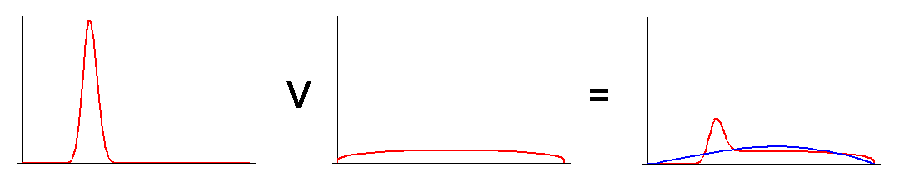
\includegraphics[scale=1.0]{A-max-B--ugly-pdf.eps}
\caption{pdf's of $z_1$, $z_2$, $max\{z_1,z_2\}$}
\end{figure}
where the blue line is the Beta distribution approximation (made by setting the mean and variance identical as the real result's).  There may also be problems when some of the input distributions $f_1(z_1),f_2(z_2),...$ are of the 'U' shape.

%If it is $min()$:\\
%\hspace*{1.2cm} $ F_0(t) = \mathbf{P}(\widetilde{\vee}(Z_1,Z_2) \leq t)$\\
%\hspace*{2cm} $\approx \mathbf{P}(min(Z_1,Z_2) \leq t)$\\
%\hspace*{2cm} $= \mathbf{P}(Z_1 \leq t \vee Z_2 \leq t)$\\
%\hspace*{3cm} assuming $Z_1, Z_2$ independent:\\
%\hspace*{2cm} $= \mathbf{P}(Z_1 \leq t) + \mathbf{P}(Z_2 \leq t) - \mathbf{P}(Z_1 \leq t) \mathbf{P}(Z_2 \leq t)$\\
%\hspace*{2cm} $= F_1(t) + F_2(t) - F_1(t) F_2(t)$

The result for $z_0 := z_1 \, \widetilde{\wedge} \, z_2$ is similar (again assuming $Z_1, Z_2$ independent):
\begin{equation}
f_0(t) \approx f_1(t) + f_2(t) - f_1(t) F_2(t) + f_2(t) F_1(t)
\end{equation}

\subsection{Cases 9-12: P(B) rule (= probability conditional)}
%This is ``Bayesian network technology''.

\textbf{Case \#9}: $\mathcal{B}$ variable\\
$\mathcal{P}$ inference --- solved in \S\ref{sec:P-inference}.

\textbf{Case \#10}: $\mathcal{Z}$ variable\\
Convert $\mathcal{Z}$ variable to $\mathcal{B}$ variable, then Case \#9.

\textbf{Case \#11}: $\mathcal{P}(\mathcal{B})$ variable\\
$\mathcal{P}$ inference --- solved in \S\ref{sec:P-inference}.

\textbf{Case \#12}: $\mathcal{P}(\mathcal{Z})$ variable\\
Convert $\mathcal{P}(\mathcal{Z})$ variable to $\mathcal{P}(\mathcal{B})$ variable, then Case \#11.

%\textcolor{red}{The stuff below this line are just my notes and may contain many errors.}
%\hrulefill

%In the probabilistic setting... we have to deal with adding rules and using the ``combination rule''... 
%
%\hspace*{1cm} \[ f = \frac{f_1 w_1 + f_2 w_2}{w_1 + w_2} \]

%The assumption is...?
%
%The confidence of the result is given by:\\
%\hspace*{1cm} \[ c = C(c_1, c_2) ? \]

%\subsection{Hybrid rules}
%\label{sec:hybrid-rules}
%
%Some rules may involve factors of various truth-value types.  For example, ``almost'' means ``close to, but not being'', which translates to this rule:\\
%\hspace*{1cm} $\mbox{almost } Q \leftarrow \mbox{ close-to } Q \wedge \neg Q$\\
%where the first factor is $\mathcal{Z}$, the second factor is $\mathcal{B}$.
%
%Maybe we should disallow $\mathcal{P}(\mathcal{Z})$-rules in the AGI because they are too sophisticated?
%
%The hybrid rules can be:\\
%\hspace*{1cm} \begin{tabular}{|l|l|l|l|l|} \hline
%                           & $\mathcal{B}$           & $\mathcal{Z}$                     & $\mathcal{P}(\mathcal{B})$ & $\mathcal{P}(\mathcal{Z})$\\ \hline
%                           & $\vee \wedge$           &                                   &            & \\
%$\mathcal{Z}$              & case H1                 & $\widetilde\vee \widetilde\wedge$ &                         & \\
%$\mathcal{P}(\mathcal{B})$ & $\curlyvee \curlywedge$ & case H2                           & $\curlyvee \curlywedge$ & \\
%$\mathcal{P}(\mathcal{Z})$ & case H3                 & case 8                            & case H4                 & $\widetilde\curlyvee \widetilde\curlywedge$ \\ \hline
%\end{tabular}
%
%TO-DO:  unfinished.

\subsection{Unified BPZ inference}
\label{sec:unified-BPZ-inference}

This section is optional.  As far as inference goes, the rest of this chapter has outlined the algorithms.  Here we try to see how $\mathcal{B}$, $\mathcal{P}$, and $\mathcal{Z}$ can be unified under the most general logic, $\mathcal{P}(\mathcal{Z})$.  Such a logic may be desirable in machine learning, where the general form of $\mathcal{P}(\mathcal{Z})$-rules may allow us to perform the searching in a continuous space, and some of the rules will degenerate nicely into $\mathcal{B}$, $\mathcal{Z}$, and $\mathcal{P}(\mathcal{B})$ rules.  Anyway, it turns out that $\mathcal{P}(\mathcal{Z})$-rules are not that simple and degeneration is also complex.

First, let's start with a general form of $\mathcal{Z}$-rule which is a function $\mathcal{Z} \times \mathcal{Z} \cdots \rightarrow \mathcal{Z}$:\\
$$ z_0 := \widetilde{\bigvee_i}\, \widetilde{\bigwedge_j}\, \Gamma_{ij}(z_{ij}) $$
where $\Gamma_{ij}$ are Gaussian functions with means $z^*_{ij}$ and variances $v_{ij}$ (in other sections we don't use the variance).  The interpretation of $\Gamma$ is:  $z^*_{ij}$ represent the optimal values, which results in $\Gamma = 1$, and when $z_{ij}$ deviates from $z^*_{ij}$, $\Gamma$ drops from 1.

Now generalize this to the $\mathcal{P}(\mathcal{Z})$-rule which is a function $\mathcal{P}(\mathcal{Z}) \times \mathcal{P}(\mathcal{Z}) \cdots \rightarrow \mathcal{P}(\mathcal{Z})$.  Let's denote $\mathcal{P}(\mathcal{Z})$ variables as $\mathbf{W}$.  Each $\mathbf{W}$ is a Beta distribution with mean $z^*$ and variance $v$.  A $\mathcal{P}(\mathcal{Z})$-rule has the general form:\\
\begin{equation}
\mathbf{W}_0 \leftarrow \widetilde{\bigcurlyvee_i} \, \widetilde{\bigcurlywedge_j}\, \Gamma_{ij}(\mathbf{W}_{ij})
\end{equation}
which contains the parameters $z^*_{ij}$, $v_{ij}$, and $c_{ij}$ (from the probabilistic $\curlyvee \curlywedge$, \S\ref{sec:probabilistic-AND-OR}).  $\widetilde{\curlyvee} \widetilde{\curlywedge}$ is different from $\widetilde{\vee} \widetilde{\wedge}$ and $\curlyvee \curlywedge$, and the rule is interpreted as follows:

\textbullet \, If the rule is $ \mathbf{W}_0 \leftarrow \Gamma_1(\mathbf{W}_1) $ we simply apply $\Gamma_1$ to the distribution $\mathbf{W}_1$.  The variance of $\mathbf{W}$ may change because of $\Gamma$.  This is covered in \hyperref[case8]{Case \#8}.

\textbullet \, Suppose the rule is $ \mathbf{W}_0 \leftarrow \mathbf{W}_1 \, \widetilde{\curlyvee} \, \mathbf{W}_2 $.  In \hyperref[case8]{Case \#8} we considered how to plug a $\mathcal{P}(\mathcal{Z})$-variable into a $\mathcal{Z}$-rule.  There, the $\mathcal{Z}$-rule did not actively affect the probability distributions.  Now the $\widetilde{\curlyvee}$ adds a constraint on the probability of $\mathbf{W}_0$ based on the values $c_1, c_2$ (from eqn (\ref{eqn:probabilistic-AND-OR})).  So we add the constraint:\\
\hspace*{1cm} $ P(z_0 = z^*_0 \, | \, z_1 = z^*_1, z_2 = z^*_2) = c_1 + c_2 - c_1 c_2 $\\
where the RHS comes from eqn (\ref{eqn:probabilistic-AND-OR}).  The effect of this is to change the shape of $\mathbf{W}_0$ to ``sharper'' or ``broader''.  The sharper the shape, and thus the smaller the variance, the more certain we are that $z_0 = z^*_0$.  But the formula is incorrect because continuous probabilities at a point is meaningless.  So we need to say\\
\hspace*{1cm} $ P(z_0 \in N(z^*_0) \, | \, z_1 \in N(z^*_1), z_2 \in N(z^*_2)) = c_1 + c_2 - c_1 c_2 $\\
where N is the interval $[0,\frac{1}{2}]$ or $[\frac{1}{2},1]$, whichever $z$ is in, thus transforming $z$ as binary.

\textbf{Degeneration of rules.}

\textbullet \, A $\mathcal{P}(\mathcal{B})$-rule reduces to a $\mathcal{B}$-rule when $c_{ij} \rightarrow 1$ (\S\ref{sec:probabilistic-AND-OR}).\\
\textbullet \, A $\mathcal{P}(\mathcal{Z})$-rule reduces to a $\mathcal{Z}$-rule when $c_{ij} \rightarrow 1$.\\
\textbullet \, A $\mathcal{Z}$-rule reduces to a $\mathcal{B}$-rule when $\Gamma_{ij} \rightarrow I$, the identity function.\\
\textbullet \, A $\mathcal{P}(\mathcal{Z})$-rule reduces to a $\mathcal{P}(\mathcal{B})$-rule when $\Gamma_{ij} \rightarrow I$.

One problem is that when we say a $\mathcal{P}$-rule degenerates into a $\mathcal{B}$-rule, it can remain to be a $\mathcal{Z}$-rule with $\Gamma_{ij} = I$.  The rule itself cannot tell us which type it is.

\section{Meta-reasoning of uncertainties}

Meta-reasoning is an important topic that will be treated in \S\ref{ch:meta-reasoning}.

One example of meta-reasoning pertinent to fuzziness is:\\
\hspace*{1cm} S1: ``You are either a patriot or a traitor.''\\
\hspace*{1cm} S2: ``No, I can be slightly patriotic or slightly traitorous.''

In S1 the predicates \textit{patriot} and \textit{traitor} are binary.  In S2 they become fuzzy.  It requires the ability for the AGI to reason \textit{about} truth-value types.

\section{PZB logic formulated as FOL axioms}

In this section I give the complete axioms for PZB logic, expressed in FOL.  That means, a FOL system will have the power of PZB logic when equipped with these axioms.  Thus, this allows us to build an AGI using a FOL inference engine as the core.

\textbf{Case \#1:}\\
(none)

\textbf{Case \#2:}\\


\textbf{Case \#3:}
\textbf{Case \#4:}
\textbf{Case \#5:}
\textbf{Case \#6:}
\textbf{Case \#7:}
\textbf{Case \#8:}
\textbf{Case \#9:}
\textbf{Case \#10:}
\textbf{Case \#11:}
\textbf{Case \#12:}

%\section{Outstanding problems}

%1. There will be many factors.  It seems that the structural organization of factors is more important than numerical curve fits.

%2. Often I feel that the numerical values aren't that important at all.  Also I feel that there are many rules that are just B -- for example, $smart \leftarrow creative$.  Even if we have a Z rule, we should be able to talk about the B counterpart.  This is very perplexing... the Z rule may take away the meta-reasoning ability of B rules...?  But the B rule will retain that ability.  Maybe the Z rule can also have the ability of meta-reasoning?  That 'creative' is a component of 'smart'?

%3. The exact form of $P(Z)$ can be irregular, especially when it is given by several factors.

%4. ``Almost P (interpreted as binary)'' is ``close to P (interpreted as Z) $\wedge$ not P (interpreted as binary)''.  So it can be a strictly-B rule with a Z-literal translated to B.  But if the Z-literal is ``not that close to P'' then ``almost P'' may be partially true.  ``Almost P'' can be slightly true, slightly not true, very true etc.  And that seems to depend on the evaluation of ``close to P''.  Because ``close to P'' can be Z, then it seems that ``almost P'' can be Z too.  

%5. The question is whether ``almost P'' is B or Z.  Maybe in various contexts it can be both?  Or may be if it is ``very almost'' then we can as well make it B.  But if it is ``slightly not almost'' then we should make it Z.

%6. The problem now seems to be that we need meta-level intervention to decide what kind of TVs to use.  But the base logic (object-level logic) has difficulty deciding on its own.  This is a problem because the base logic is not well-defined.  We need some simple rules to decide what kind of TVs to use.

%7. It's obvious we need a choice of TVs.  In the ``almost'' case... there is perhaps a distinction between base logic and meta-logic, but this distinction is orthogonal to the choice of TVs.  Maybe there is always a choice of TVs but it is too sophisticated for the base logic?  But somehow the base logic has to make a choice... 

%8. Do rules have ``intrinsic'' TVs for each slot?

%9. Another problem is how to learn B rules *gradually*?  Perhaps we start with P(B) rules and then their P's tend to $\{0,1\}$?  How about Z rules -- do they ever turn into B rules?  Maybe some of the predicates turn binary?
